% Options for packages loaded elsewhere
\PassOptionsToPackage{unicode}{hyperref}
\PassOptionsToPackage{hyphens}{url}
%
\documentclass[
  12pt,
  a5,margin=2cmpaper,
]{article}
\usepackage{amsmath,amssymb}
\usepackage{iftex}
\ifPDFTeX
  \usepackage[T1]{fontenc}
  \usepackage[utf8]{inputenc}
  \usepackage{textcomp} % provide euro and other symbols
\else % if luatex or xetex
  \usepackage{unicode-math} % this also loads fontspec
  \defaultfontfeatures{Scale=MatchLowercase}
  \defaultfontfeatures[\rmfamily]{Ligatures=TeX,Scale=1}
\fi
\usepackage{lmodern}
\ifPDFTeX\else
  % xetex/luatex font selection
\fi
% Use upquote if available, for straight quotes in verbatim environments
\IfFileExists{upquote.sty}{\usepackage{upquote}}{}
\IfFileExists{microtype.sty}{% use microtype if available
  \usepackage[]{microtype}
  \UseMicrotypeSet[protrusion]{basicmath} % disable protrusion for tt fonts
}{}
\makeatletter
\@ifundefined{KOMAClassName}{% if non-KOMA class
  \IfFileExists{parskip.sty}{%
    \usepackage{parskip}
  }{% else
    \setlength{\parindent}{0pt}
    \setlength{\parskip}{6pt plus 2pt minus 1pt}}
}{% if KOMA class
  \KOMAoptions{parskip=half}}
\makeatother
\usepackage{xcolor}
\usepackage{longtable,booktabs,array}
\usepackage{calc} % for calculating minipage widths
% Correct order of tables after \paragraph or \subparagraph
\usepackage{etoolbox}
\makeatletter
\patchcmd\longtable{\par}{\if@noskipsec\mbox{}\fi\par}{}{}
\makeatother
% Allow footnotes in longtable head/foot
\IfFileExists{footnotehyper.sty}{\usepackage{footnotehyper}}{\usepackage{footnote}}
\makesavenoteenv{longtable}
\usepackage{graphicx}
\makeatletter
\def\maxwidth{\ifdim\Gin@nat@width>\linewidth\linewidth\else\Gin@nat@width\fi}
\def\maxheight{\ifdim\Gin@nat@height>\textheight\textheight\else\Gin@nat@height\fi}
\makeatother
% Scale images if necessary, so that they will not overflow the page
% margins by default, and it is still possible to overwrite the defaults
% using explicit options in \includegraphics[width, height, ...]{}
\setkeys{Gin}{width=\maxwidth,height=\maxheight,keepaspectratio}
% Set default figure placement to htbp
\makeatletter
\def\fps@figure{htbp}
\makeatother
\setlength{\emergencystretch}{3em} % prevent overfull lines
\providecommand{\tightlist}{%
  \setlength{\itemsep}{0pt}\setlength{\parskip}{0pt}}
\setcounter{secnumdepth}{-\maxdimen} % remove section numbering
\newlength{\cslhangindent}
\setlength{\cslhangindent}{1.5em}
\newlength{\csllabelwidth}
\setlength{\csllabelwidth}{3em}
\newlength{\cslentryspacingunit} % times entry-spacing
\setlength{\cslentryspacingunit}{\parskip}
\newenvironment{CSLReferences}[2] % #1 hanging-ident, #2 entry spacing
 {% don't indent paragraphs
  \setlength{\parindent}{0pt}
  % turn on hanging indent if param 1 is 1
  \ifodd #1
  \let\oldpar\par
  \def\par{\hangindent=\cslhangindent\oldpar}
  \fi
  % set entry spacing
  \setlength{\parskip}{#2\cslentryspacingunit}
 }%
 {}
\usepackage{calc}
\newcommand{\CSLBlock}[1]{#1\hfill\break}
\newcommand{\CSLLeftMargin}[1]{\parbox[t]{\csllabelwidth}{#1}}
\newcommand{\CSLRightInline}[1]{\parbox[t]{\linewidth - \csllabelwidth}{#1}\break}
\newcommand{\CSLIndent}[1]{\hspace{\cslhangindent}#1}
\ifLuaTeX
  \usepackage{selnolig}  % disable illegal ligatures
\fi
\IfFileExists{bookmark.sty}{\usepackage{bookmark}}{\usepackage{hyperref}}
\IfFileExists{xurl.sty}{\usepackage{xurl}}{} % add URL line breaks if available
\urlstyle{same}
\hypersetup{
  pdftitle={Detection of prostate cancer in whole-slide images through end-to-end training with image-level labels},
  pdfauthor={Hans Pinckaers, Wouter Bulten, Jeroen van der Laak, Geert Litjens  },
  hidelinks,
  pdfcreator={LaTeX via pandoc}}

\title{Detection of prostate cancer in whole-slide images through
end-to-end training with image-level labels}
\author{Hans Pinckaers, Wouter Bulten, Jeroen van der Laak, Geert
Litjens \footnote{Manuscript submitted on June 6, 2020. This work was
  supported by the Dutch Cancer Society under Grant KUN 2015-7970.}
\footnote{Hans Pinckaers, Wouter Bulten, Jeroen van der Laak and Geert
  Litjens are with the Computational Pathology Group, Department of
  Pathology, Radboud Institute for Health Sciences, Radboud University
  Medical Center, Nijmegen, The Netherlands; E-mail: \{hans.pinckaers,
  wouter.bulten, jeroen.vanderlaak, geert.litjens\}@radboudumc.nl.
  Additionally, Jeroen van der Laak is with the Center for Medical Image
  Science and Visualization, Linköping University, Linköping, Sweden.}}
\date{}

\begin{document}
\maketitle
\begin{abstract}
Prostate cancer is the most prevalent cancer among men in Western
countries, with 1.1 million new diagnoses every year. The gold standard
for the diagnosis of prostate cancer is a pathologists' evaluation of
prostate tissue.

To potentially assist pathologists deep-learning-based cancer detection
systems have been developed. Many of the state-of-the-art models are
patch-based convolutional neural networks, as the use of entire scanned
slides is hampered by memory limitations on accelerator cards.
Patch-based systems typically require detailed, pixel-level annotations
for effective training. However, such annotations are seldom readily
available, in contrast to the clinical reports of pathologists, which
contain slide-level labels. As such, developing algorithms which do not
require manual pixel-wise annotations, but can learn using only the
clinical report would be a significant advancement for the field.

In this paper, we propose to use a streaming implementation of
convolutional layers, to train a modern CNN (ResNet-34) with 21 million
parameters end-to-end on 4712 prostate biopsies. The method enables the
use of entire biopsy images at high-resolution directly by reducing the
GPU memory requirements by 2.4 TB. We show that modern CNNs, trained
using our streaming approach, can extract meaningful features from
high-resolution images without additional heuristics, reaching similar
performance as state-of-the-art patch-based and multiple-instance
learning methods. By circumventing the need for manual annotations, this
approach can function as a blueprint for other tasks in
histopathological diagnosis.

The source code to reproduce the streaming models is available at
\url{https://github.com/DIAGNijmegen/pathology-streaming-pipeline}.
\end{abstract}

\hypertarget{introduction}{%
\section{Introduction}\label{introduction}}

The current state-of-the-art in computer vision for image classification
tasks are convolutional neural networks (CNNs). Commonly, convolutional
neural networks are developed with low-resolution labeled images, for
example 0.001 megapixels for CIFAR-10\textsuperscript{1}, and 0.09-0.26
megapixels for ImageNet\textsuperscript{2}. These images are evaluated
by the network and the parameters are optimized with stochastic gradient
descent by backpropagating the classification error. Neural networks
learn to extract relevant features from their input. To effectively
learn relevant features, optimizing these networks requires relatively
large datasets\textsuperscript{3}.

In histopathology, due to the gigapixel size of scanned samples,
generally referred to as whole-slide images (WSIs), the memory
limitation of current accelerator cards prohibits training on the entire
image, in contrast to most of the natural images used in general
computer vision tasks. As such, most networks are trained on tiny
patches from the whole-slide image. Acquiring labels for these patches
can be expensive. They are generally based on detailed outlines of the
classes (e.g., tumor regions) by an experienced pathologist. This
outlining is not done in clinical practice, and is a tedious and
time-consuming task. This limits the dataset size for training models.
Also, we will need to create these annotations for every individual
task.

Besides time constraints, the diagnosis also suffers from substantial
inter-observer and intra-observer variability\textsuperscript{4}. For
prostate cancer, pathologists report the Gleason grading
scheme\textsuperscript{5}. Prognostically interesting growth patterns
are categorized, resulting in three levels of aggressiveness. When
cancer is present, the reports will mention a Gleason score, a
combination of the two most informative growth patterns. These are the
most common patterns or the highest pattern. There is disagreement in
the detection of prostate cancer, as in the grading using the Gleason
scheme. Since pathologists can disagree between therapeutically relevant
growth patterns and the presence of a tumor, there are clinically
relevant consequences per individual case.

However, if we could circumvent labeling on a patch level, clinically
evaluated biopsies could be cheaply labeled using their clinical
reports. These reports contain all relevant information for clinical
decisions, and are thus of large value for machine learning algorithms.

In this paper we will focus on prostate cancer detection, determining
whether a biopsy contains cancerous glands or not. The diagnosis of
prostate cancer---the most prevalent cancer for men in Western
countries---is established by detection on histopathological slides by a
pathologist. The microscopy slides containing cross-sections of biopsies
can exhibit morphological changes to prostate glandular structures. In
low-grade tumors, the epithelial cells still form glandular structures;
however, in the case of high-grade tumors, the glandular structures are
eventually lost\textsuperscript{6}.

In the presence of cancer, the percentage of cancerous tissue in a
prostate biopsy can be as low as 1\%, the evaluation of the biopsies can
be tedious and error-prone, causing disagreement in the detection of
prostate cancer, as in the grading using the Gleason
scheme\textsuperscript{4}.

Besides substantial inter-observer and intra-observer variability,
diagnosing prostate cancer is additionally challenging due to increasing
numbers of biopsies as a result of the introduction of prostate-specific
antigen (PSA) testing\textsuperscript{7}. This number is likely to
increase further due to the aging population. In the light of a shortage
of pathologists\textsuperscript{8}, automated methods could alleviate
workload.

To reduce potential errors and workload, recent
work\textsuperscript{9--15}, has shown the potential to automatically
detect prostate cancer in biopsies. These studies either use expensive,
pixel-level annotations or train CNNs with slide-level labels only,
using a patch-based approach.

One popular strategy is based on multiple-instance-learning
(MIL)\textsuperscript{16--18}. In this approach, the whole-slide image
(WSI) is subdivided into a grid of patches. The MIL assumption states
that in a cancerous slide (`positive bag'), at least one patch will
contain tumorous tissue, whereas negative slides have no patches
containing tumour. Under this assumption, a CNN is trained on a
patch-level to find the most tumorous patch.

However, this approach has several disadvantages\textsuperscript{19}.
First, this method only works for tasks where the label can be predicted
from one individual patch and a single adversarial patch can result in a
false positive detection. Second, it is essentially a patch-based
approach, therefore, the size of the patch constrains the field-of-view
of the network.

In this paper, we propose a novel method, using
streaming\textsuperscript{20}, to train a modern CNN (ResNet-34) with 21
million parameters end-to-end to detect prostate cancer in whole-slide
images of biopsies. We also investigate the use of transfer learning
with this approach. This method does not suffer from the same
disadvantages as the aforementioned approaches based on MIL: it can use
the entire content of the whole-slide image for its prediction and the
field-of-view is not limited to an arbitrary patch-size. We compare our
approach against the methods by Campanella \emph{et
al.}\textsuperscript{10} and Bulten \emph{et al.}\textsuperscript{9}.
Since deep learning algorithm in computational pathology can suffer from
bad generalization towards other scanners\textsuperscript{21}, we
evaluated the generalization of the MIL- and streaming-trained ResNet-34
on additional biopsies acquired with a different scanner, previously
used by Litjens \emph{et al.}\textsuperscript{12}.

The streaming implementation allows us to train a convolutional neural
network directly on entire biopsy images at high-resolution (268
megapixels) using only slide-level labels. We show that a
state-of-the-art CNN can extract meaningful features from
high-resolution images using labels from pathology reports without
additional heuristics or post-processing. Subsequently, we show that
transfer learning from ImageNet performs well for images that are 5000x
bigger than the original images used for training (224x224), improving
accuracy en decreasing train time.

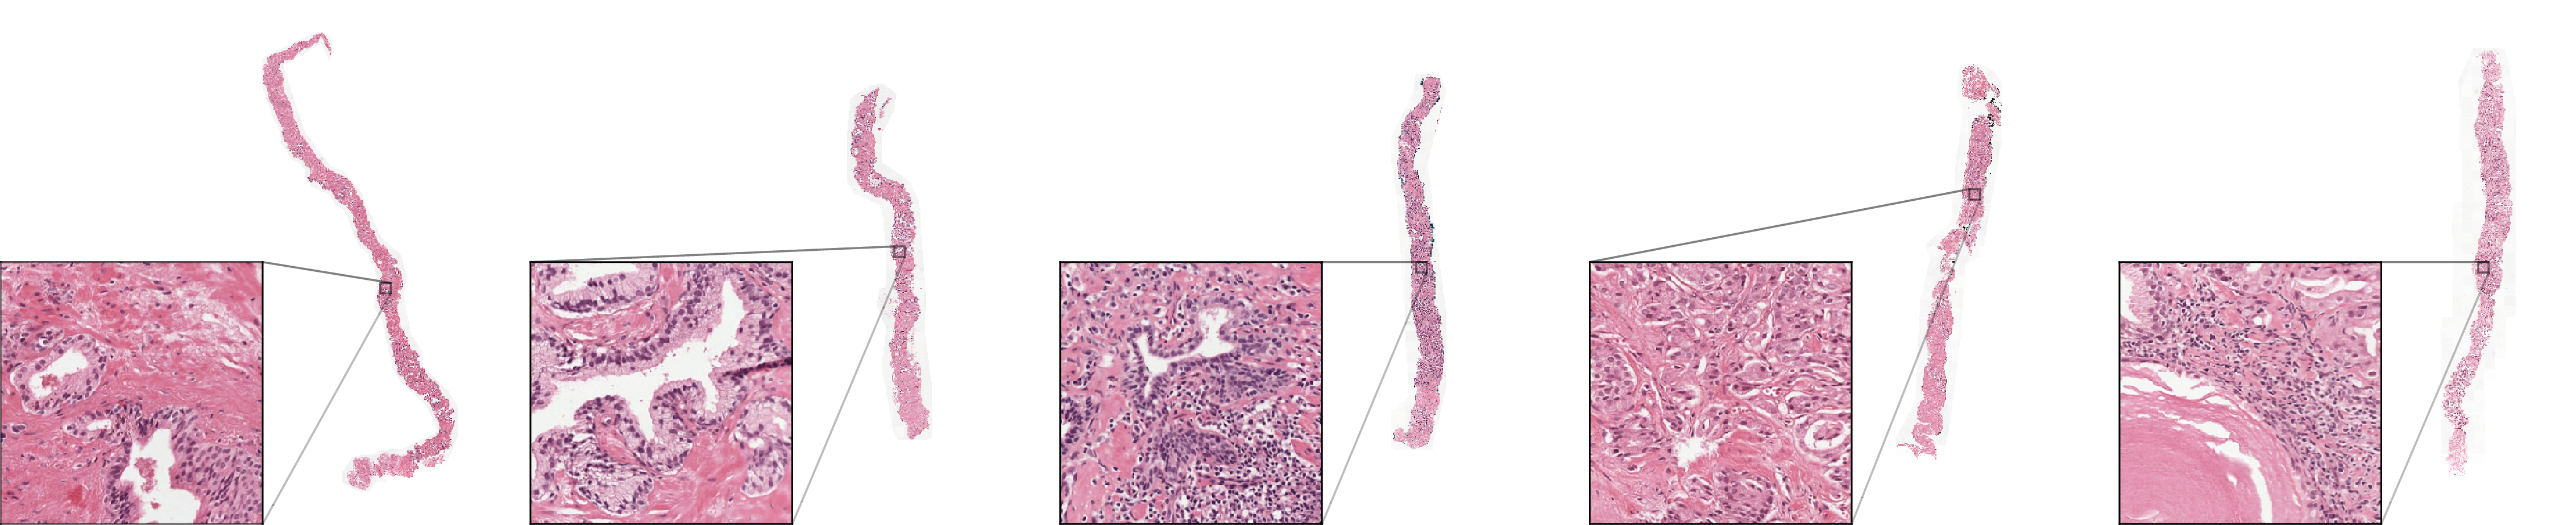
\includegraphics{chpt3_imgs/data_overview.png}

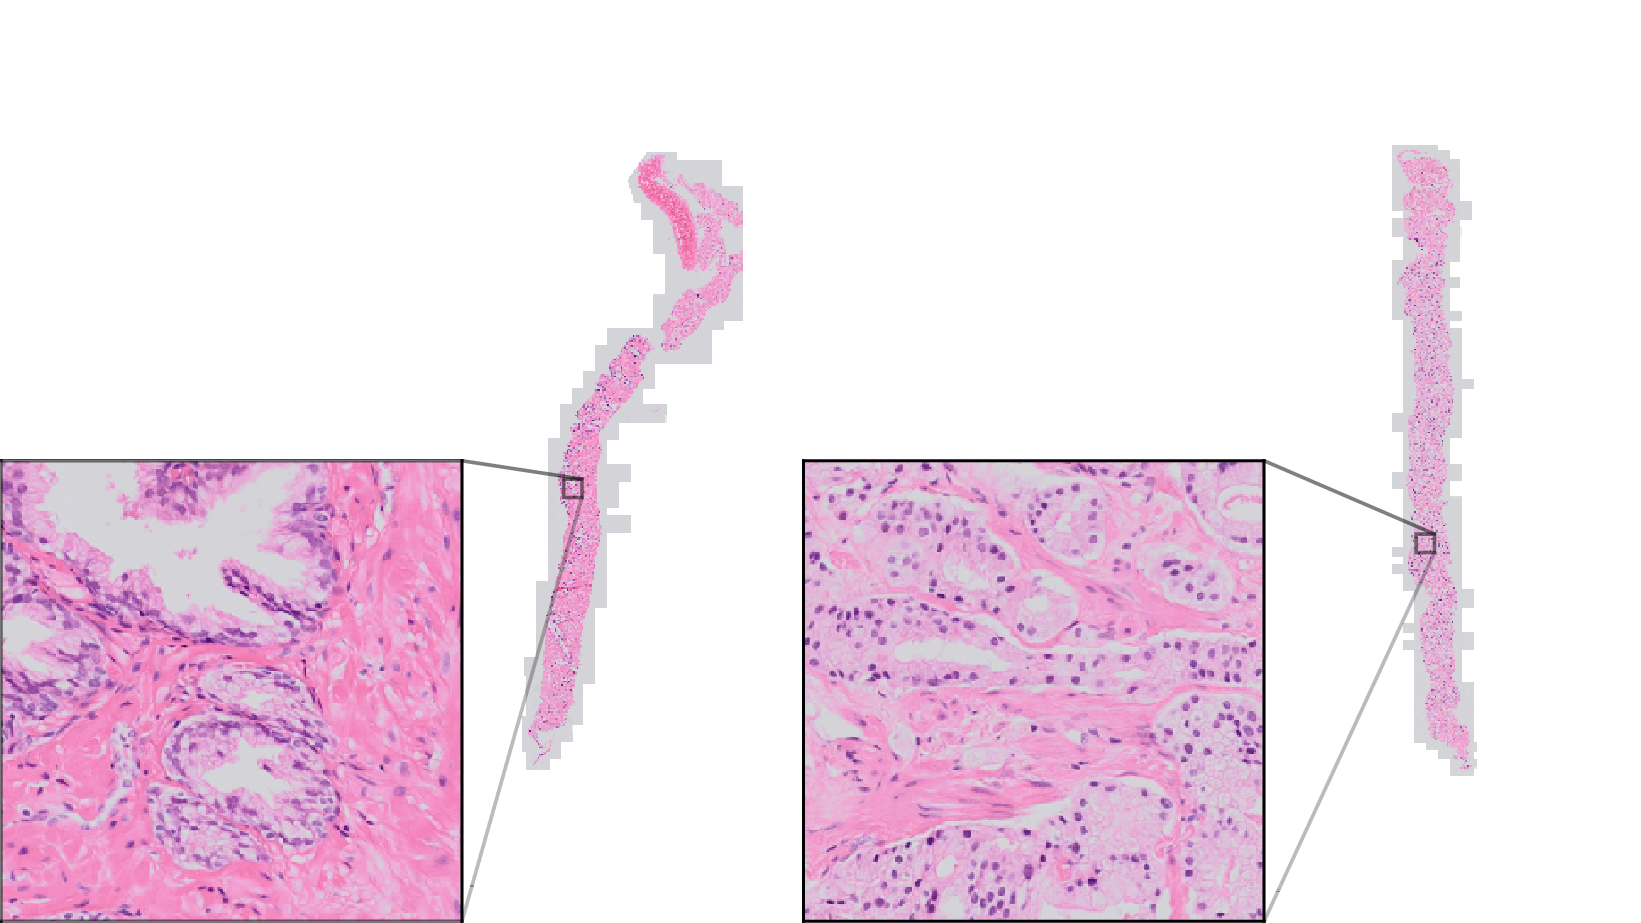
\includegraphics{chpt3_imgs/overview_olympus.png}

\hypertarget{related-works}{%
\section{Related works}\label{related-works}}

For prostate cancer detection, previous works have used more traditional
machine learning (i.e., feature-engineering)
approaches\textsuperscript{22--24}. Recently, researchers transitioned
to using deep-learning-based methods for the detection of
cancer\textsuperscript{10,12}. Besides detection, research on prostate
cancer grading has also been published\textsuperscript{9,13,14}.

In this work, we train on labels for individual biopsies. Since in other
work, the memory of the accelerator restricts the input size of the
image, published methods are based on searching relevant patches of the
original slide\textsuperscript{10,25--28}, or compressing the slide into
a smaller latent space\textsuperscript{29}.

We explicitly compare against the state-of-the-art method from
Campanella \emph{et al.}\textsuperscript{10}. As mentioned before, their
multiple-instance-learning approach is based on the single
most-informative patch, and thus leads to a small field-of-view for the
network, and potential false positives because of a few adversarial
patches. To circumvent some of these problems, Campanelle \emph{et
al.}\textsuperscript{10}, tried to increase the field-of-view to
multiple patches using a recurrent neural networks with some
improvement. Their system achieved an area-under-the-receiver-operating
curve (AUC) of 0.986. the aggregation method increased the AUC to 0.991.
To make the comparison fair, we trained a ResNet-34 network architecture
for both methods. However, when training end-to-end, the context of the
whole image is automatically taken into account.

Campanella \emph{et al.} showed that performance decreases when using
smaller datasets, concluding that at least 10,000 biopsies are necessary
for a good performance. Since they did not use data augmentation
(probably because of the big dataset at hand), we investigated if we
could reach similar performances with smaller dataset sizes using data
augmentation.

Since the mentioned implementation of multiple-instance-learning only
considers one patch, which may be less efficient,
others\textsuperscript{26,27} improved the method by using multiple
resolution patches and attention mechanisms. Li \emph{et al.} trained
two models on low and high resolution patches, only patches that were
predicted as suspicious by the lower resolution model were used to train
the higher resolution model. Additionally, to calculate the attention
mechanisms, all patches need to be kept in memory, limiting the size of
the patches. Lu \emph{et al.}\textsuperscript{26} showed that,
additionally to attention mechanisms, a frozen model pretrained on
ImageNet decreases training time and improves data efficiency. We also
use ImageNet weights, but by using the streaming-implementation of
convolutions, can unfreeze the model and train the whole network
end-to-end. However, in both papers, no comparison to the original
method of Campanella \emph{et al.} was performed.

\hypertarget{materials}{%
\section{Materials}\label{materials}}

We used the same dataset as Bulten \emph{et al.}\textsuperscript{9}, we
will briefly reiterate the collection of the dataset here. We built our
dataset by retrospectively collecting biopsies and associated pathology
reports of patients. Subsequently, we divided the patients between
training, validation, and test set. As standard practice, we optimized
the model using the training set and assessed generalization using the
validation set during development. After development, we evaluated the
model on the test set. The dataset, except for the test set, is publicly
available as a Kaggle challenge at
\url{https://www.kaggle.com/c/prostate-cancer-grade-assessment}. An
additional set, termed Olympus set, was used for evaluation with a
different scanner, originally extracted by Litjens et
al\textsuperscript{12}.

\hypertarget{data-collection}{%
\subsection{Data collection}\label{data-collection}}

We retrieved pathologists reports of prostate biopsies for patients with
a suspicion of prostate cancer, dated between Jan 1, 2012, and Dec 31,
2017, from digital patient records at the Radboud University Medical
Center, excluding patients who underwent neoadjuvant or adjuvant
therapy. The local ethics review board waived the need for informed
consent (IRB approval 2016--2275).

After anonymization, we performed a text search on the anonymized
pathology reports to divide the biopsies into positive and negative
cases. Afterward, we divided the patient reports randomly into training,
validation, and test set. By stratifying the biopsies on the primary
Gleason score, we retrieved a comparable grade distribution in all sets.
From the multiple cross-sections which were available per patient, we
selected the standard hematoxylin-and-eosin-stained glass slide
containing the most aggressive or prevalent part of malignant tissue for
scanning.

We digitized the selected glass slides using a 3DHistech Pannoramic
Flash II 250 (3DHistech, Hungary) scanner at a pixel resolution of
\(0.24 \mu m\). Since each slide could contain one to six unique
biopsies, commonly with two consecutive sections of the biopsies per
slide, trained non-experts coarsely outlined each biopsy, assigning each
with either the reported Gleason score, or labeling negative, based on
the individual biopsy descriptions in the pathology report.

We collected 1243 glass slides, containing 5759 biopsies sections. After
division, the training set consisted of 4712 biopsies, the validation
set of 497 biopsies, and the test set of 550 biopsies (Table
\protect\hyperlink{tab:extset}{1}, Fig.
\protect\hyperlink{fig:example}{{[}fig:example{]}}). We extracted the
individual biopsies from the scanned slides at a pixel resolution of
\(0.96 \mu m\), visually approximately equivalent to 100x total
magnification (i.e., 10x microscope objective with a standard 10x ocular
lens). Subsequently, we trimmed the whitespace around the tissue using a
tissue-segmentation neural network\textsuperscript{30}.

\hypertarget{reference-standard-test-set}{%
\subsection{Reference standard test
set}\label{reference-standard-test-set}}

To determine a strong reference standard, three specialized pathologists
reviewed the slides in three rounds. In the first round, each
pathologist graded the biopsies independently. In the second round, each
biopsy for which no consensus was reached in the first round, consensus
was regraded by the pathologist whose score differed from the other two,
with the help of the pathologist's first score and the two anonymous
Gleason scores of the other pathologists. In the third round, the
pathologists discussed the biopsies without consensus after round two.
In total 15 biopsies were discarded by the panel as they could not be
reliably graded, resulting in a total test set size of 535 biopsies.
See\textsuperscript{9} for a complete overview of the grading protocol.

\hypertarget{smaller-subsampled-training-set}{%
\subsection{Smaller subsampled training
set}\label{smaller-subsampled-training-set}}

To test our method with smaller datasets, we sampled 250 (5\%) and 500
(10\%) biopsies from the training set. Half of the cases in the new sets
were negatives. For the positive biopsies, we stratified on primary
Gleason grade and sampled equal amounts of each. Thus, we kept the
distribution of the positive biopsies equal over all the datasets. We
used the 5\% (250 biopsies) and 10\% (500 biopsies) datasets for
training. The validation- and test-sets were equal to the ones used in
the development of the model on the whole set.

\hypertarget{tab:extset}{}
\begin{longtable}[]{@{}llllll@{}}
\caption{Distribution of datasets used in the experiments, stratisfied
on primary Gleason pattern.}\tabularnewline
\toprule\noalign{}
\textbf{Dataset} & \textbf{Total} & \textbf{Negative} & \textbf{3} &
\textbf{4} & \textbf{5} \\
\midrule\noalign{}
\endfirsthead
\toprule\noalign{}
\textbf{Dataset} & \textbf{Total} & \textbf{Negative} & \textbf{3} &
\textbf{4} & \textbf{5} \\
\midrule\noalign{}
\endhead
\bottomrule\noalign{}
\endlastfoot
Training set & 4712 & 16\% & 32\% & 45\% & 7\% \\
Validation set & 497 & 39\% & 23\% & 29\% & 9\% \\
10\% set & 500 & 50\% & 17\% & 17\% & 17\% \\
5\% set & 250 & 51\% & 16\% & 16\% & 16\% \\
Test set & 535 & 47\% & 25\% & 19\% & 9\% \\
Olympus set & 205 & 58\% & 25\% & 11\% & 4\% \\
\end{longtable}

\hypertarget{olympus-set}{%
\subsection{Olympus set}\label{olympus-set}}

For the Olympus set, we used the slides of Litjens \emph{et al.},
2016\textsuperscript{12}. That set contained 255 glass slides, scanned
using an Olympus VS120-S5 system (Olympus, Japan). In comparison to the
original paper, we used all biopsies on a negative slide, instead of
only one, resulting in 291 biopsies (Fig.
\protect\hyperlink{fig:olympusexample}{{[}fig:olympusexample{]}}). Since
patients in this set were biopsied in 2012, there was a small overlap
with the primary dataset used in this paper. We excluded 86 biopsies
from 53 duplicate patients, resulting in a set of 205 biopsies.

\hypertarget{methods}{%
\section{Methods}\label{methods}}

\hypertarget{end-to-end-streaming-model}{%
\subsection{End-to-end streaming
model}\label{end-to-end-streaming-model}}

We trained a ResNet-34\textsuperscript{31} convolutional neural network.
Since the individual biopsy images differ in size, we padded or
center/cropped them to 16384\(\times\)16384 input. 99\% of our dataset
biopsies fitted within this input size. Since padding small biopsies
results in a lot of whitespace, we changed the final pooling layer of
ResNet-34 to a global max-pool layer.

For regularization, we used extensive data augmentation. To make
augmentation of these images feasible with reasonable memory usage and
speed, we used the open-source library VIPS\textsuperscript{32}. Elastic
random transformation, color augmentation (hue, saturation, and
brightness), random horizontal and vertical flipping, and rotations were
applied. We normalized the images based on training dataset statistics.

We initialized the networks using ImageNet-trained weights. As an
optimizer, we used standard SGD (learning rate of \(2e-4\)) with
momentum (0.9) and a mini-batch size of 16 images. Because when using
streaming, we do not have a full image on the GPU, we cannot use batch
normalization, thus we froze the batch normalization mean and variance,
using the transfer-learned ImageNet running mean and variance. We
randomly oversampled negative cases to counter the imbalance in the
dataset\textsuperscript{33}.

For the experiments with random weights, we initialized the networks
using He \emph{et al.}\textsuperscript{34}. We also used mixed precision
training\textsuperscript{35} to speed up training since these networks
needed more epochs to convergence.

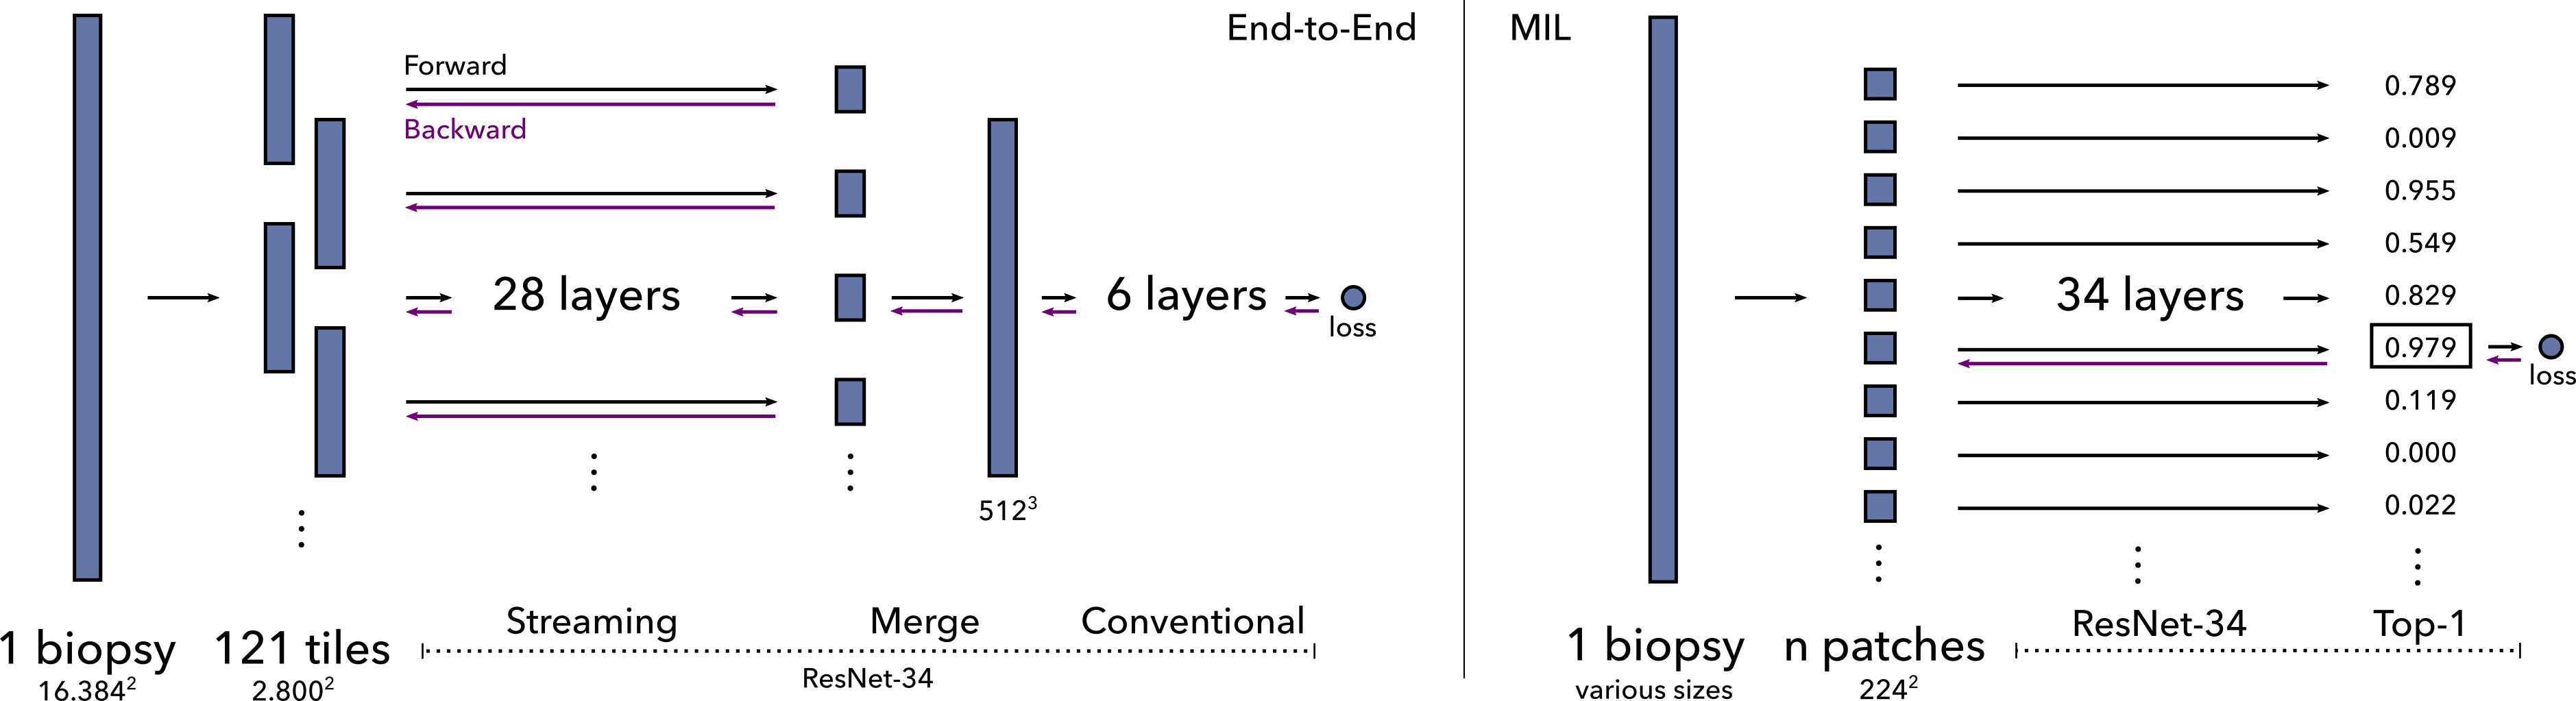
\includegraphics{chpt3_imgs/methods_overview_cropped.png}

\hypertarget{streaming-cnn}{%
\subsubsection{Streaming CNN}\label{streaming-cnn}}

Most convolutional neural network architectures trained for a
classification task require more memory in the first layers than in the
latter because of the large feature maps. Our previously published
method termed `streaming'\textsuperscript{20} circumvents these high
memory requirements in the first layers by performing the operations on
a tile-by-tile basis. This method is possible because CNNs use small
kernels; hence the result at any given location is only defined by a
small area of the input. This area is called the field-of-view. Since
the field-of-view at the beginning of a network is vastly smaller than
the full input image, we can use tiles (which have to be bigger than the
field-of-view) to perform the convolutions serially. Thereby only
requiring the amount of memory for the calculation on a single tile
instead of the whole input image. After streaming, we concatenate the
tile outputs to retrieve the complete intermediate feature map of the
last streamed layer. This complete feature map is equal to the feature
map we would get when training on a infinite-memory GPU.

During the forward pass of these memory-heavy first layers, we keep the
final layer output and remove the output of the other intermediate
layers, to save memory. We stream as many layers as needed until the
last streamed layer's output can fit into GPU memory. This feature map
can subsequently be fed through the rest of the neural network at once,
resulting in the final output.

For the backward pass, we can use a similar implementation. The last
layers, until the last streamed layer, can be backpropagated as usual.
Then, we correctly tile the gradient of the last streamed layer's
output. We use these gradient tiles for tile-by-tile backpropagation of
the streamed layers. Leveraging the input tile, we recalculate the first
layers' intermediate feature maps with a forward pass (this is commonly
called gradient checkpointing\textsuperscript{36}. With the recalculated
features and the gradient tile, we can finish the backpropagation for
the respective tile. We perform this for every tile. This way, we can
recover the gradients of all parameters, as would be the case if
training with the original input image. See Figure
\protect\hyperlink{figure:streamingSGD}{{[}figure:streamingSGD{]}} for a
graphical representation of the methods.

To train the ResNet-34, we streamed with a tile size of
2800\(\times\)2800 (Fig.
\protect\hyperlink{fig:memrelation}{{[}fig:memrelation{]}}) over the
first 28 layers of the network. After these layers, the whole feature
map (with dimensions 512\(\times\)512\(\times\)512) could fit into GPU
memory. It is possible to use the streaming implementation for more
layers of the network, however, to improve speed it is better to stream
until the feature map is just small enough. Finally, we fed the map
through the remaining six layers to calculate the final output.

For the experiments with random weights in mixed precision, due to the
decrease in memory usage, we could use a tile size of 3136\(\times\)3136
to increase speed, and decrease the number of streamed layers to the
first 27.

\hypertarget{training-schedule}{%
\subsubsection{Training schedule}\label{training-schedule}}

In transfer learning, often the first layers are treated as a feature
extraction algorithm. After the feature extraction part, the second part
is trained for the specific task\textsuperscript{37}. Since the domain
of histopathology differs significantly from the natural images in
ImageNet, we froze the first three (of the four) residual blocks of the
network (the first 27 layers) as feature extractor, only training the
last block for our task. This also has the benefit of training faster,
since we do not need to calculate gradients for the first layers. After
25 epochs, all the networks were stabilized and stopped improving the
validation loss, showing slightly lower train losses.

From these epochs, we picked a checkpoint with a low validation loss to
resume fine-tuning the whole network, unfreezing the weights of the
first three residual blocks. Due to the relatively small validation set,
the loss curve was less smooth than the training loss curve. To account
for a sporadic checkpoint with a low loss, we calculated a moving
average over five epochs. From these averages, we picked the window with
the lowest loss, taking the middle checkpoint of the averaging window.

Starting from this checkpoint, we fine-tuned the whole network with a
learning rate of \(6e-5\). After approximately 50 epochs, all the
networks stopped improving. For inference, we choose the checkpoints
based on a moving average of five epochs with the lowest validation set
loss. We averaged the weights of these checkpoints to improve
generalization\textsuperscript{38}.

For the streaming experiments with random weights, we used the exact
same training schedule except for the learning rate. The loss would go
to infinity in the first few batches. When training from scratch, we
could not use the first layers as feature extractor. We fine-tuned the
whole network with a learning rate of \(1e-5\) requiring 100 epochs
until the validation loss did stabilized. We subsequently lowered the
learning rate to \(3e-6\) for 200 epochs after which the validation loss
stopped improving.

The optimization and training procedure was fully conducted using the
validation set, the test set, and the Olympus set were untouched during
the development of the model.

\hypertarget{gradient-accumulation-and-parallelization}{%
\subsubsection{Gradient accumulation and
parallelization}\label{gradient-accumulation-and-parallelization}}

Gradient accumulation is a technique to do a forward and backward pass
on multiple images in series on the accelerator card, and averaging the
parameter gradients over those images. Only after averaging, we perform
a gradient descent step. Averaging the gradients over multiple images in
series results in effectively training a mini-batch of these multiple
images, while only requiring the memory for one image at a time. We used
gradient accumulation over multiple biopsies to achieve an effective
mini-batch size of 16 images.

We trained over multiple GPUs by splitting the mini-batch. For the
streaming experiments, we used four GPUs (either NVIDIA RTX 2080ti or
GTX 1080ti).

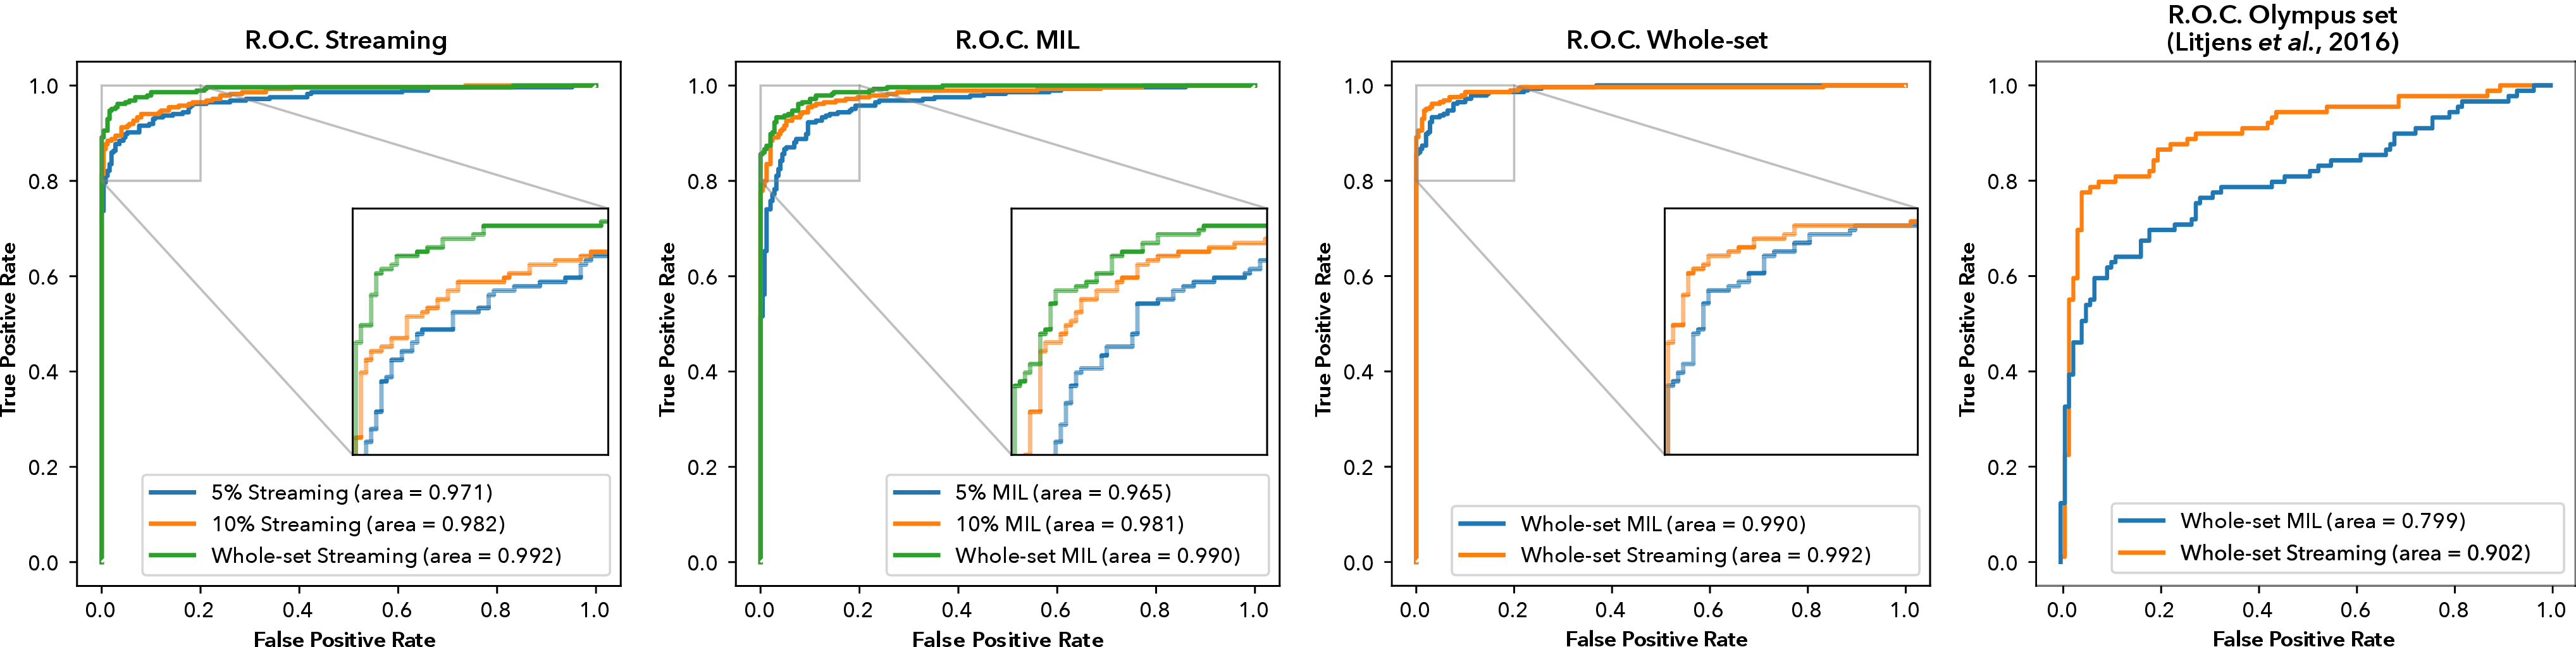
\includegraphics{chpt3_imgs/auc_both.png}

\hypertarget{multiple-instance-learning-model}{%
\subsection{Multiple-instance-learning
model}\label{multiple-instance-learning-model}}

As a baseline, we implemented the multiple-instance-learning method as
described in\textsuperscript{10}.

This method divides the images into a grid of smaller patches with the
assumption that an individual patch could determine the image-level
label. The task is to find the most informative patch. In our binary
detection task, the most informative patch is determined by the patch
with the highest probability of tumor. If there is a patch with a high
probability of tumorous tissue, the whole biopsy is labeled tumorous.

We train such a model, per epoch, in two phases. The first phase is the
inference phase, where we process all the patches of a biopsy, thereby
finding the patch with the highest probability. This patch gets assigned
the image-level label. Then, in the training phase, using only patches
with the highest probability (the top-1 patch), the model parameters are
optimized with a loss calculated on the patch probability and the label.

We followed the implementation from Campanella \emph{et
al.}\textsuperscript{10}, but tweaked it for our dataset sizes. We used
standard SGD (learning rate of \(1e-5\)) with momentum (0.9) with a
mini-batch size of 16 images. We froze the BatchNormalization mean and
variance, due to the smaller mini-batch size and to keep the features
equal between the inference phase and the training phase. Equally, we
oversampled negative cases to counter the imbalance in the dataset,
instead of weighting\textsuperscript{33}.

We updated the whole model for 100 epochs when transfer learning, and
200 epochs when training from random weights. From these epochs, we
picked the checkpoint with the lowest loss using the same scheme as the
streaming model. Afterward, we trained for another 100 epochs with a
learning rate of \(3e-6\). The networks trained from random
initialization on the 10\% and 5\% required 300 epochs. We again choose
the checkpoint based on the lowest validation set loss, using a moving
average of 5 epochs. We also used weight averaging for these
checkpoints.

For regularization, we used the same data augmentation as the streaming
model. We made sure that the same augmented patch was used in the
inferencing and training phase. We used ImageNet statistics to normalize
the patches.

\hypertarget{quantitative-evaluation}{%
\subsection{Quantitative evaluation}\label{quantitative-evaluation}}

The quantitative evaluation of both methods is performed using
receiver-operating characteristic (ROC) analysis. Specifically, we look
at the area under the ROC curve. To calculate a confidence interval, we
used bootstrapping. We sampled the number of the biopsies in the set,
with replacement, and calculated the area under the
receiver-operating-curve based on the new sample. Repeating this
procedure 10.000 times resulted in a distribution from which we
calculated the 95\% confidence interval (2.5 and 97.5 percentile)

\hypertarget{qualitative-evaluation}{%
\subsection{Qualitative evaluation}\label{qualitative-evaluation}}

To assess the correlation of certain regions to the cancerous label, we
created heatmaps for both techniques. For MIL, we used the patch
probabilities. For streaming, we used sensitivity maps using
SmoothGrad\textsuperscript{39}. As implementation of SmoothGrad, we
averaged 25 sensitivity maps on Gaussian-noise-augmented versions of a
biopsy. We used a standard deviation of 5\% of the image-wide standard
deviation for the Gaussian noise. As a comparison, we show pixel-level
segmentations from the model published in Bulten \emph{et
al.}\textsuperscript{9} as well.

In addition, we did a thorough analysis of the false positives and
negatives of both the MIL and the streaming methods.

\hypertarget{experiments}{%
\section{Experiments}\label{experiments}}

We performed three experiments for both methods using three datasets.
One experiment on all the data, and two on subsampled training sets, the
10\% (500 biopsies) and 5\% (250 biopsies) datasets.

\hypertarget{tab:test_results}{}
\begin{longtable}[]{@{}lll@{}}
\caption{Area under the receiver-operating-curve comparison between the
methods on the test set, \emph{trained using transfer
learning}.}\tabularnewline
\toprule\noalign{}
\textbf{Dataset} & \textbf{Method} & \textbf{AUC} \\
\midrule\noalign{}
\endfirsthead
\toprule\noalign{}
\textbf{Dataset} & \textbf{Method} & \textbf{AUC} \\
\midrule\noalign{}
\endhead
\bottomrule\noalign{}
\endlastfoot
Whole set & Streaming & 0.992 (0.985--0.997) \\
& MIL & 0.990 (0.984--0.995) \\
& Bulten \emph{et al.}\textsuperscript{9} & 0.990 (0.982--0.996) \\
10\% set & Streaming & 0.982 (0.972--0.990) \\
& MIL & 0.981 (0.970--0.990) \\
5\% set & Streaming & 0.971 (0.960--0.982) \\
& MIL & 0.965 (0.949--0.978) \\
Olympus set & Streaming & 0.909 (0.863--0.949) \\
& MIL & 0.799 (0.732--0.861) \\
\end{longtable}

\hypertarget{tab:test_results_scratch}{}
\begin{longtable}[]{@{}lll@{}}
\caption{Area under the receiver-operating-curve comparison between the
methods on the test set, \emph{trained from random
initialization}.}\tabularnewline
\toprule\noalign{}
\textbf{Dataset} & \textbf{Method} & \textbf{AUC} \\
\midrule\noalign{}
\endfirsthead
\toprule\noalign{}
\textbf{Dataset} & \textbf{Method} & \textbf{AUC} \\
\midrule\noalign{}
\endhead
\bottomrule\noalign{}
\endlastfoot
Whole set & Streaming & 0.967 (0.952--0.980) \\
& MIL & 0.918 (0.894--0.941) \\
10\% set & Streaming & 0.924 (0.900--0.945) \\
& MIL & 0.899 (0.871--0.924) \\
5\% set & Streaming & 0.915 (0.889--0.939) \\
& MIL & 0.862 (0.831--0.892) \\
\end{longtable}

On the whole dataset, the streaming model achieved an AUC of 0.992
(0.985--0.997) and the MIL model an AUC of 0.990 (0.984--0.995).
Interestingly, our models trained on the whole dataset reached similar
performance to previous work on this dataset\textsuperscript{9}, which
utilized a segmentation network trained using dense annotations obtained
in a semi-supervised fashion.

For streaming, the performance on the smaller dataset sizes are similar
between the two. 5\% dataset has an AUC of 0.971 (0.960--0.982) for 5\%
and 0.982 (0.972--0.990) for 10\% (Table
\protect\hyperlink{tab:test_results}{2}). The models trained with more
data generalize better (Fig.
\protect\hyperlink{figure:ROCcomparison}{{[}figure:ROCcomparison{]}}).

Also for multiple-instance learning there is a clear improvement going
from a model trained on the smallest dataset size, with an AUC of 0.965
(0.949--0.978), increasing to 0.981 (0.970--0.990) on the 10\% dataset.

There seems to be a trend that the MIL model performs slightly worse
(Fig.
\protect\hyperlink{figure:ROCcomparison}{{[}figure:ROCcomparison{]}}),
however, this difference falls within the confidence intervals.

In the experiments trained from random weights, there is a larger
separation between the methods, without overlap of the confidence
intervals. Streaming achieves an AUC of 0.967 (0.952--0.980) when using
the whole set (Table \protect\hyperlink{tab:test_results_scratch}{3}) in
comparison to MIL with 0.918 (0.894--0.941). For the 10\% set using
streaming also results in higher metrics 0.924 (0.900--0.945) versus
0.899 (0.871--0.924). Finally, the 5\% set gets an AUC of 0.915
(0.889--0.939) for streaming and 0.862 (0.831--0.892) for MIL.

In general, the areas identified by MIL and streaming in the heatmaps
correspond well to the pixel-level segmentations from Bulten \emph{et
al.}, showing that both methods pick up the relevant regions for cancer
identification (Figure
\protect\hyperlink{fig:heatmaps}{{[}fig:heatmaps{]}}). Most errors of
the models seem to be due to normal epithelium mimicking tumorous glands
in the case for false positives, and the small size of some tumorous
regions as a possible reason for the false negatives. (Table
\protect\hyperlink{tab:errors}{4})

For the Olympus set, existing of biopsies scanned by the Olympus
VS-system, there is a larger separation between the methods. Streaming
reaches an AUC of 0.909 (0.863--0.949), with MIL scoring 0.799
(0.732--0.861). For this dataset, MIL has 36 false negatives versus 20
for streaming, and 8 false positive versus 5 from streaming.

Identified by the MIL model.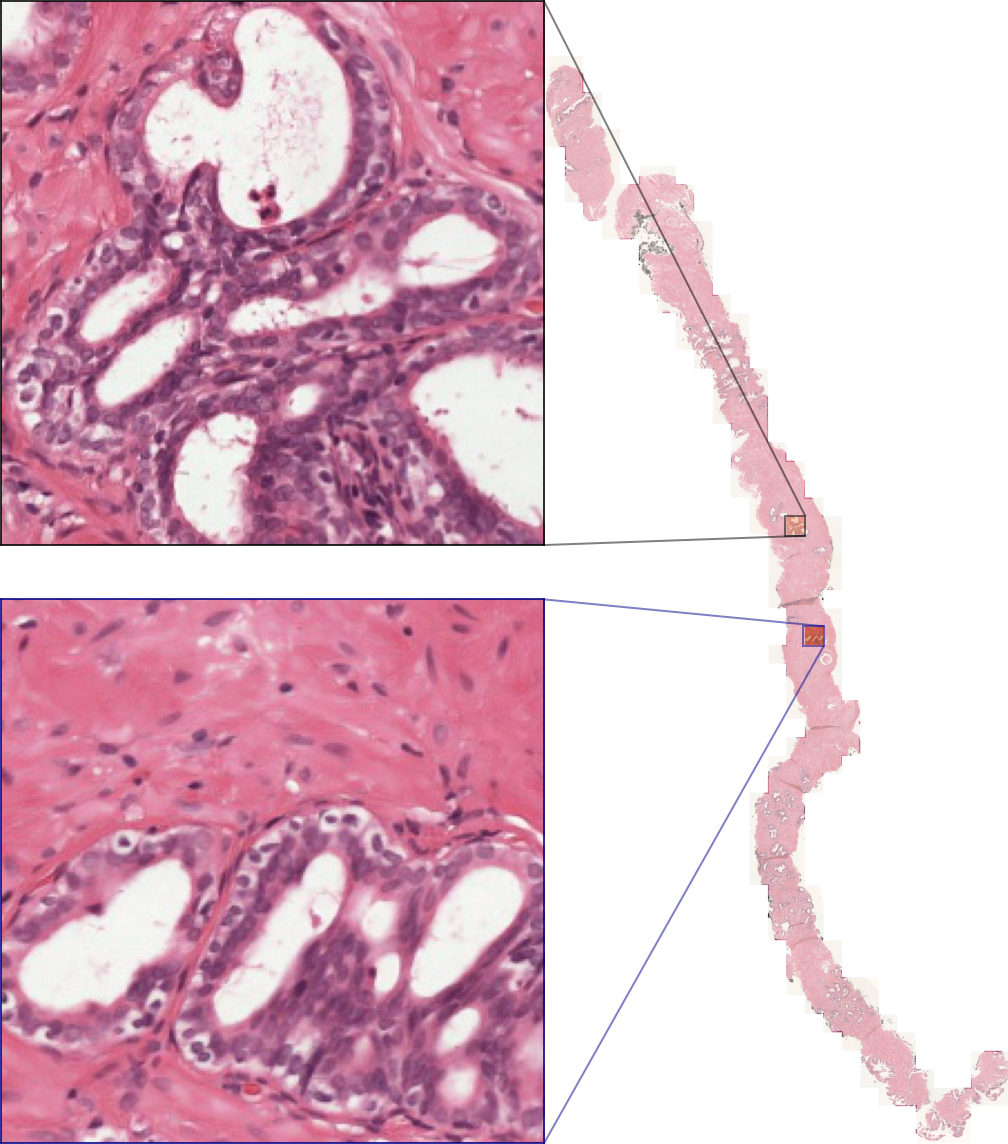
\includegraphics{chpt3_imgs/FP_MIL_1.png}
Identified by the streaming
model.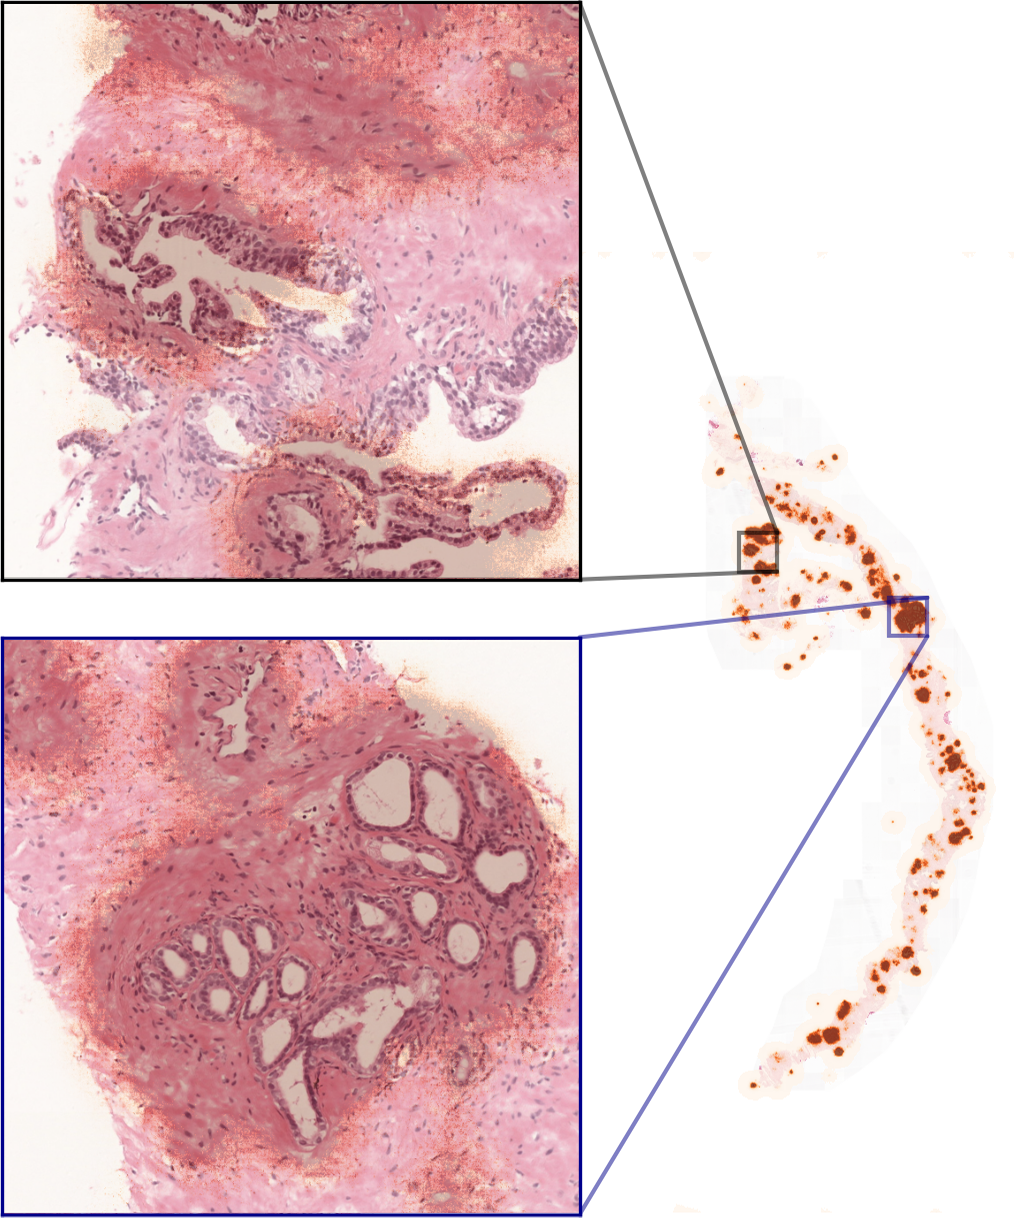
\includegraphics{chpt3_imgs/FP_e2e_1.png}

Small tumorous glands mimicking vessels. Missed by both
models.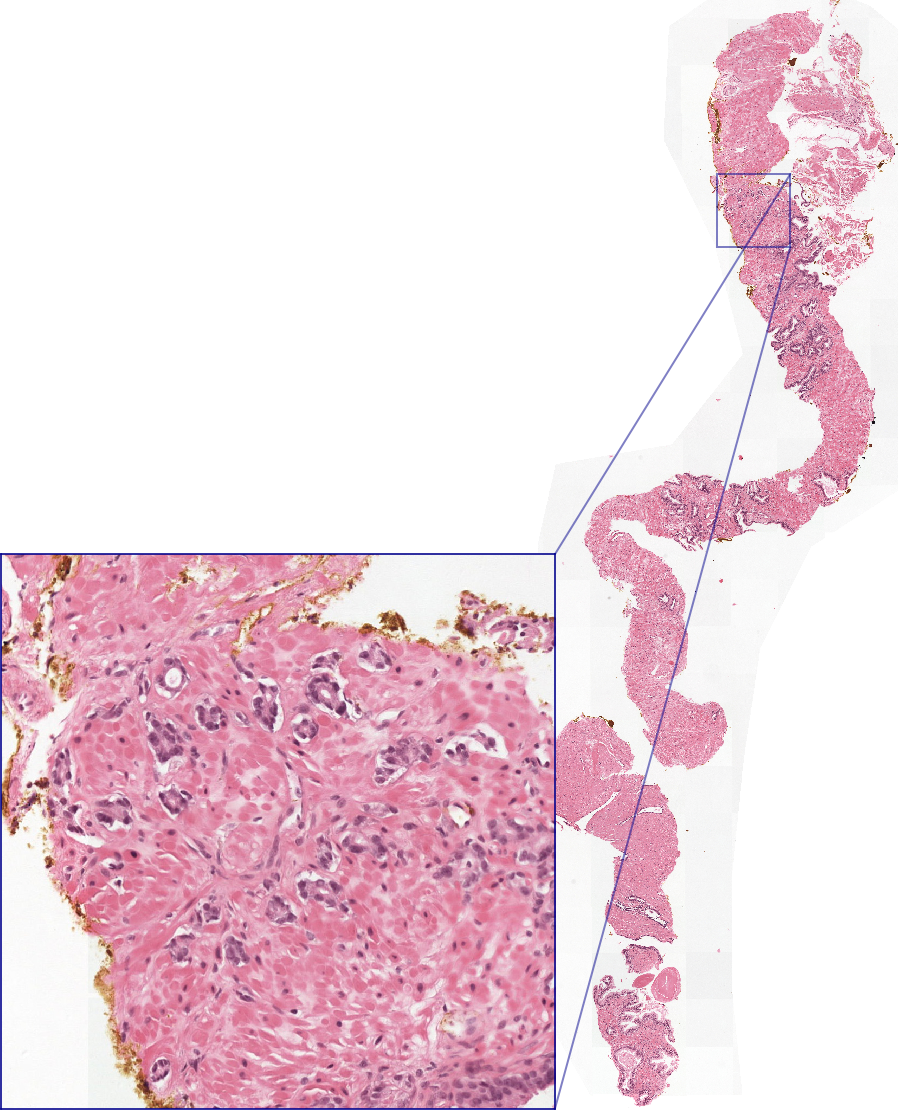
\includegraphics{chpt3_imgs/both_missed_FN.png} Very limited
amount of tumor (four glands), missed by the streaming
network.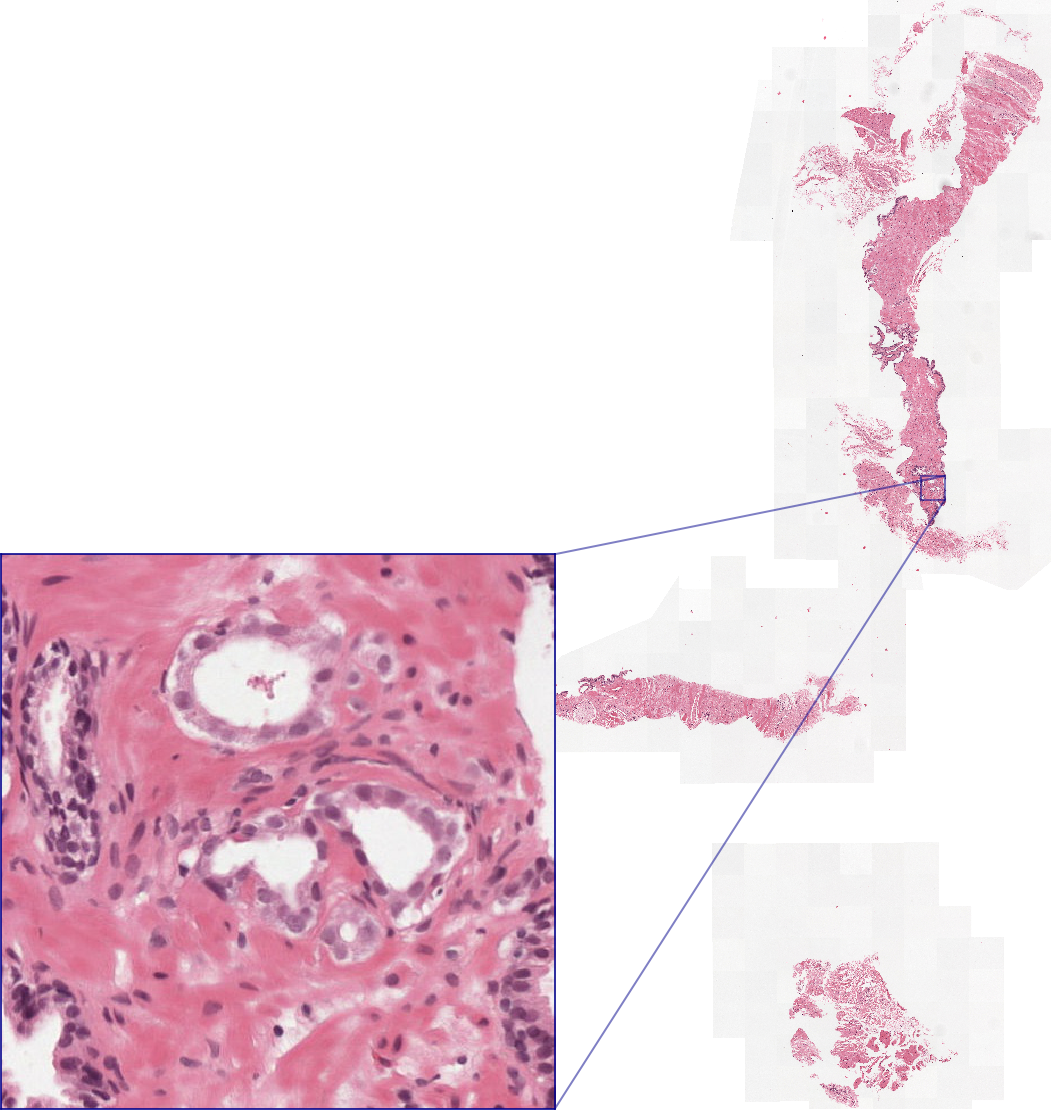
\includegraphics{chpt3_imgs/e2e_FN.png}

\hypertarget{tab:errors}{}
\begin{longtable}[]{@{}lll@{}}
\caption{The predictions were manually judged and divided in the
following categories. False positives and negatives were selected at the
point of maximum accuracy in the ROC curve.}\tabularnewline
\toprule\noalign{}
\textbf{False positives} & \textbf{Streaming} (5) & \textbf{MIL} (13) \\
\midrule\noalign{}
\endfirsthead
\toprule\noalign{}
\textbf{False positives} & \textbf{Streaming} (5) & \textbf{MIL} (13) \\
\midrule\noalign{}
\endhead
\bottomrule\noalign{}
\endlastfoot
Normal mimicking tumor & 2 & 7 \\
Inflammation & 1 & 4 \\
Tissue artefacts & 1 & 1 \\
Bladder epithelium & 1 & 0 \\
Colon epithelium & 0 & 1 \\
\textbf{False negatives} & \textbf{Streaming} (13) & \textbf{MIL}
(12) \\
Little amount of tumor & 7 & 4 \\
Tissue artefacts & 3 & 1 \\
Low-grade tumor & 1 & 2 \\
Inflammation-like & 1 & 2 \\
Unclear reason & 1 & 2 \\
\end{longtable}

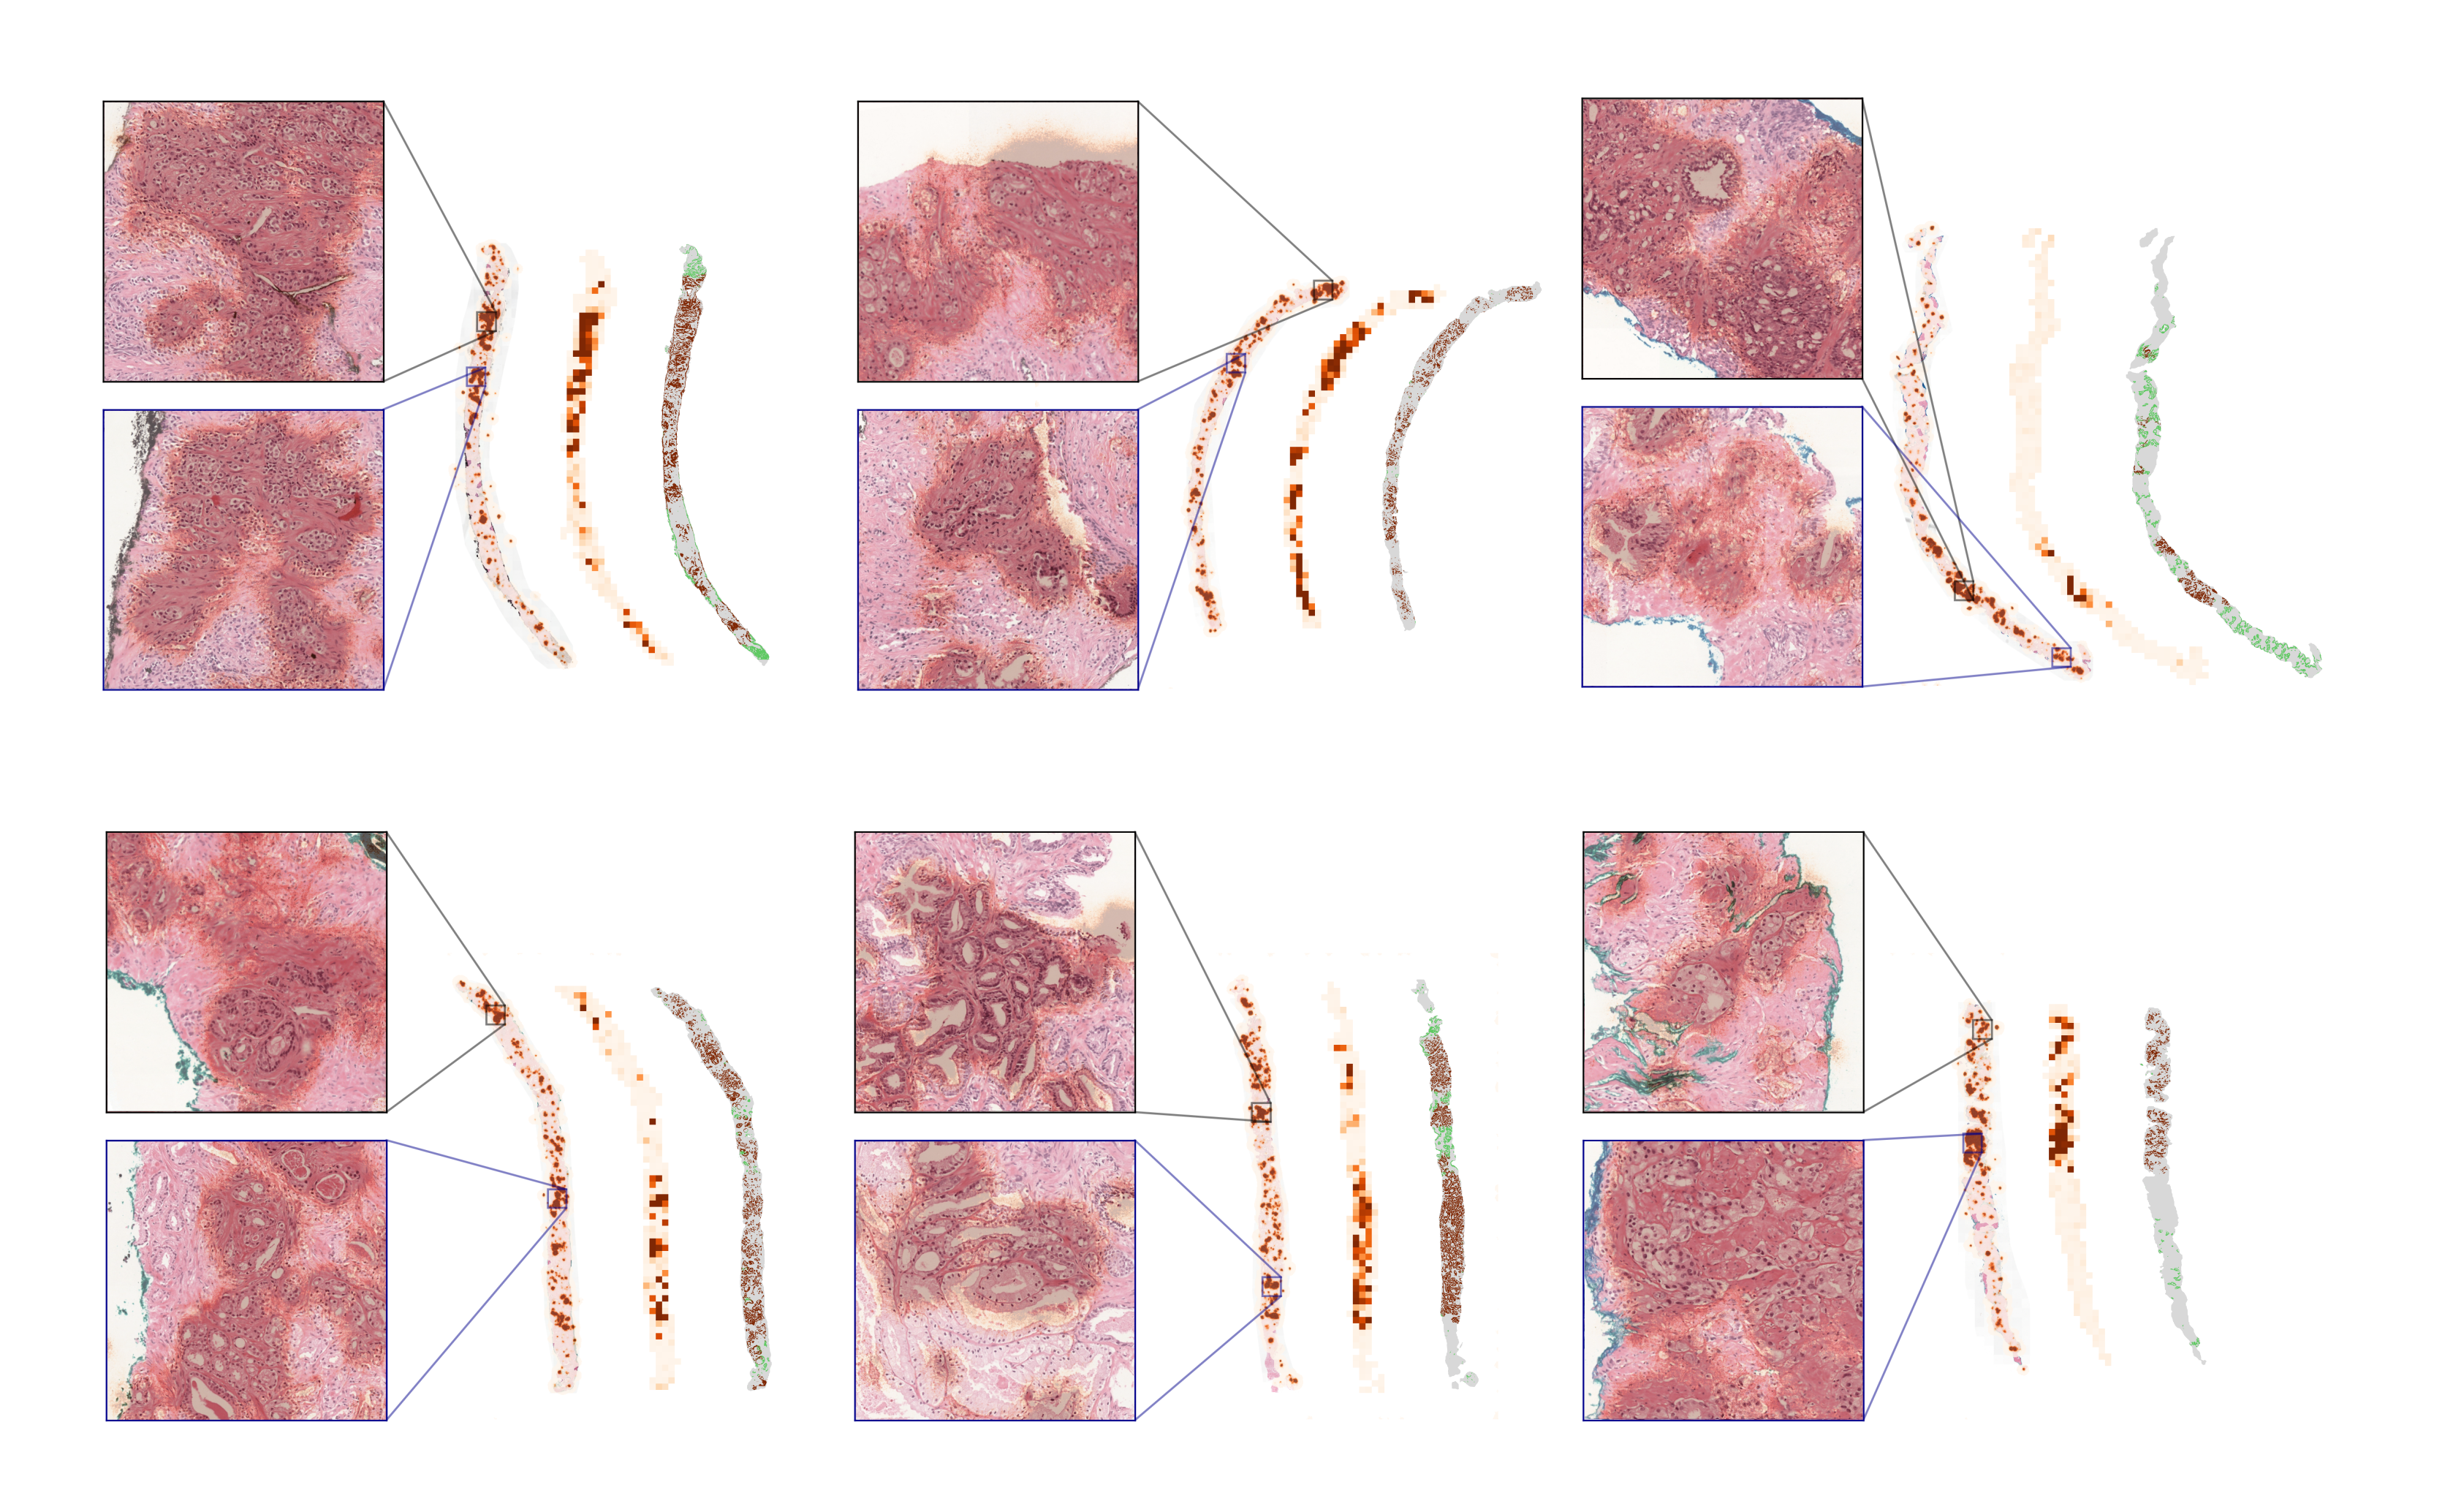
\includegraphics{chpt3_imgs/saliency_maps_darker.png}

\hypertarget{tab:times}{}
\begin{longtable}[]{@{}llll@{}}
\caption{When fine-tuning only the last six of the ResNet-34 are
trained, all other layers are frozen. All metrics are in seconds.
Preprocessing times not shown, in our experiments they accounted for 8
seconds for new biopsies. Mixed precision streaming is relatively fast
due to bigger tile-size and one less layer to stream.}\tabularnewline
\toprule\noalign{}
& \textbf{Training} & \textbf{Fine-tuning} & \textbf{Inferencing} \\
\midrule\noalign{}
\endfirsthead
\toprule\noalign{}
& \textbf{Training} & \textbf{Fine-tuning} & \textbf{Inferencing} \\
\midrule\noalign{}
\endhead
\bottomrule\noalign{}
\endlastfoot
Full precision streaming & 32.3 s & 12.5 s & 8.5 s \\
Mixed precision streaming & 17.2 s & 3.6 s & 3.5 s \\
MIL & 0.5 s & n.a. & 0.25 s \\
\end{longtable}

\hypertarget{discussion-and-conclusions}{%
\section{Discussion and conclusions}\label{discussion-and-conclusions}}

In this paper, we proposed using streaming\textsuperscript{20}
convolution neural networks to directly train a state-of-the-art
ResNet-34 architecture on whole prostate biopsies with slide-level
labels from pathology reports. We are the first to train such
high-resolution (268 megapixels) images end-to-end, without further
heuristics. Accomplishing this without the streaming implementation
would require a accelerator card with 2.4 terabyte of memory.

We showed it is possible to train a residual neural network with biopsy
level labels and reach similar performance to a popular
multiple-instance-learning (MIL) based method. Our models trained on the
whole dataset reached an AUC of 0.992 for streaming training, and 0.990
for MIL. In addition, we achieved equal performance to a method trained
on patch-based labels, with an AUC of 0.990\textsuperscript{9} on the
same dataset. Although, it should be noted that Bulten \emph{et al.}
used weakly-supervised labels, they used a cascade of models to go from
epithelium antibody-staining to semi-automatic pixel-level annotations,
to generate a model trained at the patch level.

Looking at the failure cases (Table \protect\hyperlink{tab:errors}{4}),
multiple-instance-learning suffers from interpreting normal glands as
tumorous (Fig. \protect\hyperlink{fig:errors_pos}{{[}fig:errors\_pos{]}}
and \protect\hyperlink{fig:errors_neg}{{[}fig:errors\_neg{]}}). We
hypothesize this is due to the lack of context, in all but three cases
the misclassification was due to one patch. For false negatives, both
models fail when there is a small amount of tumor, however the streaming
model seems to suffer more from this. A possible solution would be to
incorporate attention mechanisms into the network, allowing it to focus
to smaller parts of the biopsy.

To study the benefits of transfer learning, we trained the networks from
randomly initialized weights according to He \emph{et
al.}\textsuperscript{34}. These networks took longer to converge
(approximately 3-4x more iterations needed) and reached lower
performances. In this case, MIL is less capable of extracting relevant
information from the patches and scores worse than networks trained with
streaming, scoring an AUC of 0.918 versus 0.959, respectively. We think
training from random weights introduced additional noise in the
MIL-training process. Since some biopsies contain cancerous tissue that
only falls within a few patches, ImageNet weights can provide a better
starting point to find these relevant patches during training. However,
when training from random initialization, the noise of the benign
patches in a cancerous biopsy may make it harder to learn. When
possible, we advise the usage of pretrained network to increase
convergence speed and final performance.

MIL performs weaker than the streaming network on the Olympus set, with
the main error being misclassifying 36 biopsies with tumor as negative.
The external dataset has other color characteristics due to the
different scanner used. Since both network have been trained with the
same data augmentation, MIL seems to benefit less from this augmentation
thus generalizing worse. The improvement seen in generalization on the
Olympus set and the trend of higher performance overall suggest that
streaming extracts more meaningful features from the same dataset.

In this paper, we compared against a MIL implementation of Campanella
\emph{et al.} In their MIL implementation, only the top-1 patch is used
for training per epoch. The method's data efficiency is reliant on how
often different patches are selected in the first phase. Our results on
the smallest dataset sample (5\%, 250 slides) hint towards reduced data
efficiency for MIL. However, the performance on the smaller datasets was
already close to optimal, suggesting effective use of the transferred
ImageNet-weights. Even though it is not the same test set as in their
original paper, this seems to suggest a better performance for smaller
datasets than Campanella \emph{et al.} reported. Hypothetically, this
could be due to data augmentation, which they did not use, and increased
randomness with smaller mini-batch size in our study.

For MIL, selecting different patches per image, every epoch, is
important to circumvent overfitting. We used lower minibatch-sizes, 16
vs 512, and learning rates, \(1e-5\) vs \(1e-4\) as the original
implementation\textsuperscript{10}. We saw increased stability in
training using smaller mini-batch sizes and learning rates, especially
for the smaller datasets, where the whole dataset would otherwise fit in
one mini-batch. Lower mini-batch sizes increased some noise, thereby
picking different patches per epoch.

The streaming implementation of convolutional neural networks is
computationally slower than our baseline. Mainly due to the number (121)
and overlap (\textasciitilde650 pixels) of the tiles during
backpropagation. For inference new slides, taking into account the
preprocessing that needs to happen (roughly 8 seconds for extracting
patches or extracting the whole biopsy), MIL takes half the time (8.25
seconds) compared to streaming (16.5 seconds) (Table IV). The most
significant difference lies in the train speed, where for full
precision, streaming is \textasciitilde65 times slower than MIL (Table
\protect\hyperlink{tab:times}{5}). Streaming did require half the number
of epochs needed to converge, but the gap is still large. However, an
algorithm only needs to be trained once, and the inference speed for
both streaming and MIL is fast enough for use in clinical practice.

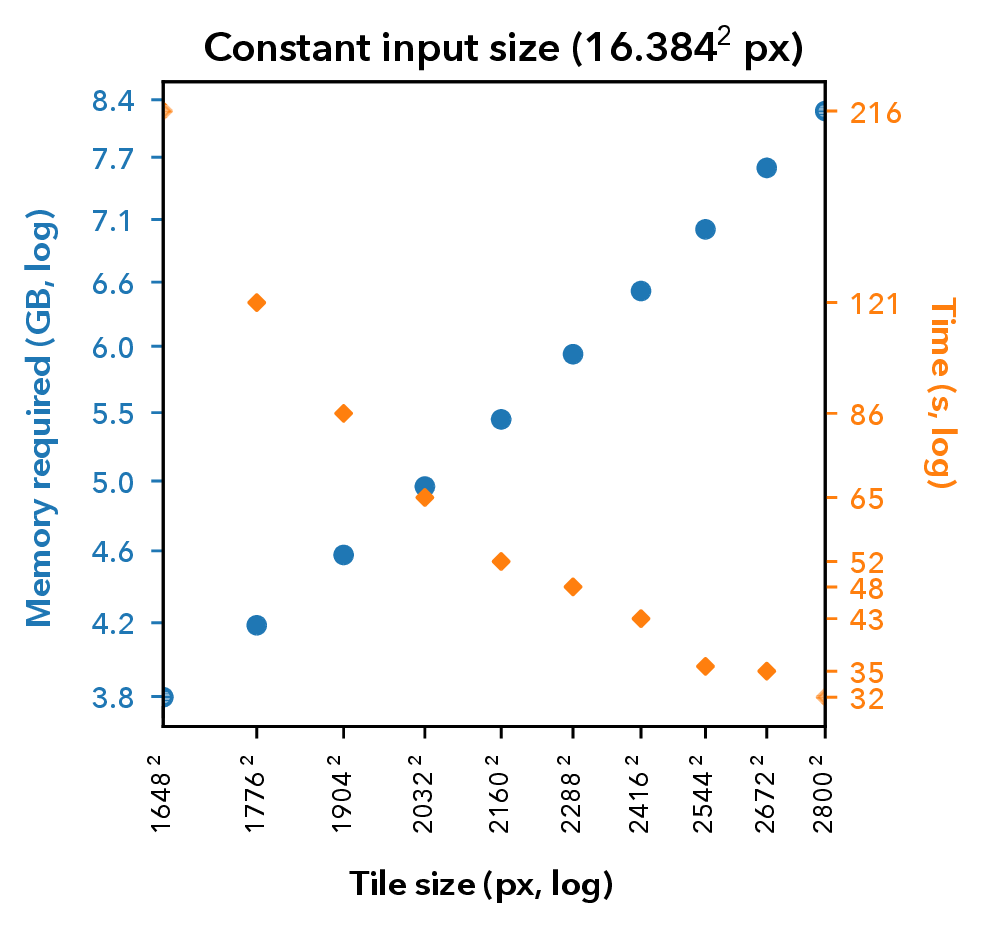
\includegraphics{chpt3_imgs/timevsmemory_final.png}

Improving the speed of the streaming implementation of convolutional
operations is of interest. In this work, we improved training speed by
first freezing the first layers of the neural network, not having to
calculate gradients. Using this training scheme in the
multiple-instance-learning baseline resulted in unstable training and
worse performance. Further research could focus on decreasing the number
of calculations needed by using variable input sizes\footnote{An example
  implementation of this can be found in the open source repository.} or
lower-level implementations that ignore whitespace, such as sparse
implementations of convolutions\textsuperscript{40}.

Streaming training with high-resolution images opens up the possibility
to quickly gather large datasets with labels from pathology reports to
train convolutional neural networks. Although linking individual
biopsies to the pathology report is still a manual task, it is more
efficient than annotating the individual slides. However, some pathology
labs will manufacture one slide per biopsy and report systematically on
these individual biopsies. Training from a whole slide, with multiple
biopsies, is left for future research.

Since multiple-instance-learning, in the end, predicts the final label
on a single patch, tasks that require information from different sites
of the biopsy could be hard to engineer in this framework. For example,
in the Gleason grading scheme, the two most informative growth patterns
are reported. These patterns could lie on different parts of the biopsy,
outside of the field-of-view of a single patch. Also, additional growth
patterns could be present. The first reported growth pattern of Gleason
grading is the most prevalent. Since multiple-instance-learning works
patch-based, volumes that span larger than one patch are not used for
the prediction. Streaming allows for training complex tasks, such as
cancer grading, even with slide-level labels.

Our heatmaps show that indeed the streaming model uses information from
multiple regions in the biopsy (Fig.
\protect\hyperlink{fig:heatmaps}{{[}fig:heatmaps{]}}). Even though our
model is not trained on a patch-level, the sensitivity maps highlight
similar regions as the MIL method and the segmentation algorithm from
Bulten \emph{et al.} Thus, interestingly, a modern convolutional neural
network, originally developed for tiny input sizes, can extract useful
information from 268 megapixel images.

Besides allowing the entire slide to inform predictions, streaming
training also has the advantage of being able to learn with hard or
impossible to annotate global information. For example, in the medical
domain, survival prediction can be of great interest. Future work could
be to predict survival from histopathology tissue directly. Reliably
annotating for this task can be difficult. Since streaming can find
patterns and features from the whole image using just the retrospective
patient prognosis, this method can be beneficial in automatically
finding new relevant biomarkers.

We provide source code of the streaming pipeline at GitHub\footnote{\url{https://github.com/DIAGNijmegen/pathology-streaming-pipeline}}.
We tried to make it easy to use with other datasets. Additionally to
methods used in this paper, we added mixed precision support for even
more memory efficient and faster training.

\hypertarget{refs}{}
\begin{CSLReferences}{0}{0}
\leavevmode\vadjust pre{\hypertarget{ref-Krizhevsky2009}{}}%
\CSLLeftMargin{1. }%
\CSLRightInline{Krizhevsky A. \emph{{Learning Multiple Layers of
Features from Tiny Images}}. University of Toronto; 2009.}

\leavevmode\vadjust pre{\hypertarget{ref-Russakovsky2015}{}}%
\CSLLeftMargin{2. }%
\CSLRightInline{Russakovsky O, Deng J, Su H, et al. {ImageNet Large
Scale Visual Recognition Challenge}. \emph{International Journal of
Computer Vision}. 2015;115(3):211-252.
doi:\href{https://doi.org/10.1007/s11263-015-0816-y}{10.1007/s11263-015-0816-y}}

\leavevmode\vadjust pre{\hypertarget{ref-Sun2017RevisitingUE}{}}%
\CSLLeftMargin{3. }%
\CSLRightInline{Sun C, Shrivastava A, Singh S, Gupta A. {Revisiting
Unreasonable Effectiveness of Data in Deep Learning Era}. \emph{2017
IEEE International Conference on Computer Vision (ICCV)}. Published
online 2017:843-852.}

\leavevmode\vadjust pre{\hypertarget{ref-Ozkan2016}{}}%
\CSLLeftMargin{4. }%
\CSLRightInline{Ozkan TA, Eruyar AT, Cebeci OO, Memik O, Ozcan L,
Kuskonmaz I. {Interobserver variability in Gleason histological grading
of prostate cancer}. \emph{Scandinavian Journal of Urology}.
2016;50(6):420-424.
doi:\href{https://doi.org/10.1080/21681805.2016.1206619}{10.1080/21681805.2016.1206619}}

\leavevmode\vadjust pre{\hypertarget{ref-Epstein2010}{}}%
\CSLLeftMargin{5. }%
\CSLRightInline{Epstein JI. {An Update of the Gleason Grading System}.
\emph{Journal of Urology}. 2010;183(2):433-440.
doi:\href{https://doi.org/10.1016/j.juro.2009.10.046}{10.1016/j.juro.2009.10.046}}

\leavevmode\vadjust pre{\hypertarget{ref-Fine2012}{}}%
\CSLLeftMargin{6. }%
\CSLRightInline{Fine SW, Amin MB, Berney DM, et al. {A contemporary
update on pathology reporting for prostate cancer: Biopsy and radical
prostatectomy specimens}. \emph{European Urology}. 2012;62(1):20-39.
doi:\href{https://doi.org/10.1016/j.eururo.2012.02.055}{10.1016/j.eururo.2012.02.055}}

\leavevmode\vadjust pre{\hypertarget{ref-10.1093ux2fjnciux2fdjp278}{}}%
\CSLLeftMargin{7. }%
\CSLRightInline{Welch HG, Albertsen PC. {Prostate Cancer Diagnosis and
Treatment After the Introduction of Prostate-Specific Antigen Screening:
1986--2005}. \emph{JNCI: Journal of the National Cancer Institute}.
2009;101(19):1325-1329.
doi:\href{https://doi.org/10.1093/jnci/djp278}{10.1093/jnci/djp278}}

\leavevmode\vadjust pre{\hypertarget{ref-Wilson2018}{}}%
\CSLLeftMargin{8. }%
\CSLRightInline{Wilson ML, Fleming KA, Kuti MA, Looi LM, Lago N, Ru K.
{Access to pathology and laboratory medicine services: a crucial gap.}
\emph{Lancet (London, England)}. 2018;391(10133):1927-1938.
doi:\href{https://doi.org/10.1016/S0140-6736(18)30458-6}{10.1016/S0140-6736(18)30458-6}}

\leavevmode\vadjust pre{\hypertarget{ref-Bulten2020}{}}%
\CSLLeftMargin{9. }%
\CSLRightInline{Bulten W, Pinckaers H, Boven H van, et al. {Automated
deep-learning system for Gleason grading of prostate cancer using
biopsies: a diagnostic study}. \emph{The Lancet Oncology}.
2020;21(2):233-241.
doi:\href{https://doi.org/10.1016/S1470-2045(19)30739-9}{10.1016/S1470-2045(19)30739-9}}

\leavevmode\vadjust pre{\hypertarget{ref-Campanella2019}{}}%
\CSLLeftMargin{10. }%
\CSLRightInline{Campanella G, Hanna MG, Geneslaw L, et al.
{Clinical-grade computational pathology using weakly supervised deep
learning on whole slide images}. \emph{Nature Medicine}.
2019;25(8):1301-1309.
doi:\href{https://doi.org/10.1038/s41591-019-0508-1}{10.1038/s41591-019-0508-1}}

\leavevmode\vadjust pre{\hypertarget{ref-Nagpal2019}{}}%
\CSLLeftMargin{11. }%
\CSLRightInline{Nagpal K, Foote D, Liu Y, et al. {Development and
validation of a deep learning algorithm for improving Gleason scoring of
prostate cancer}. \emph{npj Digital Medicine}. 2019;2(1):48.
doi:\href{https://doi.org/10.1038/s41746-019-0112-2}{10.1038/s41746-019-0112-2}}

\leavevmode\vadjust pre{\hypertarget{ref-Litjens2016}{}}%
\CSLLeftMargin{12. }%
\CSLRightInline{Litjens G, Sánchez CI, Timofeeva N, et al. {Deep
learning as a tool for increased accuracy and efficiency of
histopathological diagnosis}. \emph{Scientific Reports}.
2016;6(1):26286.
doi:\href{https://doi.org/10.1038/srep26286}{10.1038/srep26286}}

\leavevmode\vadjust pre{\hypertarget{ref-Arvaniti2018}{}}%
\CSLLeftMargin{13. }%
\CSLRightInline{Arvaniti E, Fricker KS, Moret M, et al. {Automated
Gleason grading of prostate cancer tissue microarrays via deep
learning}. \emph{Scientific Reports}. 2018;8(1):12054.
doi:\href{https://doi.org/10.1038/s41598-018-30535-1}{10.1038/s41598-018-30535-1}}

\leavevmode\vadjust pre{\hypertarget{ref-Lucas2019}{}}%
\CSLLeftMargin{14. }%
\CSLRightInline{Lucas M, Jansen I, Savci-Heijink CD, et al. {Deep
learning for automatic Gleason pattern classification for grade group
determination of prostate biopsies}. \emph{Virchows Archiv}.
2019;475(1):77-83.
doi:\href{https://doi.org/10.1007/s00428-019-02577-x}{10.1007/s00428-019-02577-x}}

\leavevmode\vadjust pre{\hypertarget{ref-Strom2020}{}}%
\CSLLeftMargin{15. }%
\CSLRightInline{Ström P, Kartasalo K, Olsson H, et al. {Artificial
intelligence for diagnosis and grading of prostate cancer in biopsies: a
population-based, diagnostic study}. \emph{The Lancet Oncology}.
2020;21(2):222-232.
doi:\href{https://doi.org/10.1016/S1470-2045(19)30738-7}{10.1016/S1470-2045(19)30738-7}}

\leavevmode\vadjust pre{\hypertarget{ref-Courtiol2018}{}}%
\CSLLeftMargin{16. }%
\CSLRightInline{Courtiol P, Tramel EW, Sanselme M, Wainrib G.
{Classification and Disease Localization in Histopathology Using Only
Global Labels: A Weakly-Supervised Approach}. \emph{arXiv preprint}.
2018;1802.02212. \url{http://arxiv.org/abs/1802.02212}}

\leavevmode\vadjust pre{\hypertarget{ref-Ilse2018}{}}%
\CSLLeftMargin{17. }%
\CSLRightInline{Ilse M, Tomczak JM, Welling M. {Attention-based Deep
Multiple Instance Learning}. \emph{arXiv preprint}. 2018;1802.04712.
\url{http://arxiv.org/abs/1802.04712}}

\leavevmode\vadjust pre{\hypertarget{ref-Amores2013}{}}%
\CSLLeftMargin{18. }%
\CSLRightInline{Amores J. {Multiple instance classification: Review,
taxonomy and comparative study}. \emph{Artificial Intelligence}.
2013;201:81-105.
doi:\href{https://doi.org/10.1016/j.artint.2013.06.003}{10.1016/j.artint.2013.06.003}}

\leavevmode\vadjust pre{\hypertarget{ref-VanderLaak2019}{}}%
\CSLLeftMargin{19. }%
\CSLRightInline{Laak J van der, Ciompi F, Litjens G. {No pixel-level
annotations needed}. \emph{Nature Biomedical Engineering}.
2019;3(11):855-856.
doi:\href{https://doi.org/10.1038/s41551-019-0472-6}{10.1038/s41551-019-0472-6}}

\leavevmode\vadjust pre{\hypertarget{ref-Pinckaers2019}{}}%
\CSLLeftMargin{20. }%
\CSLRightInline{Pinckaers H, Ginneken B van, Litjens G. {Streaming
convolutional neural networks for end-to-end learning with
multi-megapixel images}. \emph{arXiv preprint}. 2019;1911.04432.
\url{https://arxiv.org/abs/1911.04432}}

\leavevmode\vadjust pre{\hypertarget{ref-Swiderska-Chadaj2020}{}}%
\CSLLeftMargin{21. }%
\CSLRightInline{Swiderska-Chadaj Z, Bel T de, Blanchet L, et al. {Impact
of rescanning and normalization on convolutional neural network
performance in multi-center, whole-slide classification of prostate
cancer}. \emph{Scientific Reports}. 2020;10(1):14398.
doi:\href{https://doi.org/10.1038/s41598-020-71420-0}{10.1038/s41598-020-71420-0}}

\leavevmode\vadjust pre{\hypertarget{ref-Gertych2015}{}}%
\CSLLeftMargin{22. }%
\CSLRightInline{Gertych A, Ing N, Ma Z, et al. {Machine learning
approaches to analyze histological images of tissues from radical
prostatectomies}. \emph{Computerized Medical Imaging and Graphics}.
2015;46:197-208.
doi:\href{https://doi.org/10.1016/j.compmedimag.2015.08.002}{10.1016/j.compmedimag.2015.08.002}}

\leavevmode\vadjust pre{\hypertarget{ref-nguyen2017}{}}%
\CSLLeftMargin{23. }%
\CSLRightInline{Nguyen TH, Sridharan S, Macias V, et al. {Automatic
Gleason grading of prostate cancer using quantitative phase imaging and
machine learning}. \emph{Journal of biomedical optics}.
2017;22(3):36015.}

\leavevmode\vadjust pre{\hypertarget{ref-Naik2007}{}}%
\CSLLeftMargin{24. }%
\CSLRightInline{Naik S, Doyle S, Feldman M, Tomaszewski J, Madabhushi A.
{Gland Segmentation and Computerized Gleason Grading of Prostate
Histology by Integrating Low- , High-level and Domain Specific
Information.} In: \emph{Proceedings of 2nd Workshop on Microsopic Image
Analysis with Applications in Biology}.; 2007:1-8.}

\leavevmode\vadjust pre{\hypertarget{ref-Ianni2020}{}}%
\CSLLeftMargin{25. }%
\CSLRightInline{Ianni JD, Soans RE, Sankarapandian S, et al. {Tailored
for Real-World: A Whole Slide Image Classification System Validated on
Uncurated Multi-Site Data Emulating the Prospective Pathology Workload}.
\emph{Scientific Reports}. 2020;10(1):3217.
doi:\href{https://doi.org/10.1038/s41598-020-59985-2}{10.1038/s41598-020-59985-2}}

\leavevmode\vadjust pre{\hypertarget{ref-lu2020data}{}}%
\CSLLeftMargin{26. }%
\CSLRightInline{Lu MY, Williamson DFK, Chen TY, Chen RJ, Barbieri M,
Mahmood F. {Data Efficient and Weakly Supervised Computational Pathology
on Whole Slide Images}. \emph{arXiv preprint}. 2020;2004.09666.
\url{https://arxiv.org/abs/2004.09666}}

\leavevmode\vadjust pre{\hypertarget{ref-Li2019a}{}}%
\CSLLeftMargin{27. }%
\CSLRightInline{Li J, Li W, Gertych A, Knudsen BS, Speier W, Arnold CW.
{An attention-based multi-resolution model for prostate whole slide
imageclassification and localization}. \emph{arXiv preprint}.
2019;1905.13208. \url{http://arxiv.org/abs/1905.13208}}

\leavevmode\vadjust pre{\hypertarget{ref-Caner2018}{}}%
\CSLLeftMargin{28. }%
\CSLRightInline{Mercan C, Aksoy S, Mercan E, Shapiro LG, Weaver DL,
Elmore JG. {Multi-Instance Multi-Label Learning for Multi-Class
Classification of Whole Slide Breast Histopathology Images}. \emph{IEEE
Transactions on Medical Imaging}. 2018;37(1):316-325.
doi:\href{https://doi.org/10.1109/TMI.2017.2758580}{10.1109/TMI.2017.2758580}}

\leavevmode\vadjust pre{\hypertarget{ref-Tellez2019}{}}%
\CSLLeftMargin{29. }%
\CSLRightInline{Tellez D, Litjens G, Laak J van der, Ciompi F. {Neural
Image Compression for Gigapixel Histopathology Image Analysis}.
\emph{IEEE Transactions on Pattern Analysis and Machine Intelligence}.
in press.
doi:\href{https://doi.org/10.1109/TPAMI.2019.2936841}{10.1109/TPAMI.2019.2936841}}

\leavevmode\vadjust pre{\hypertarget{ref-Bandi2019a}{}}%
\CSLLeftMargin{30. }%
\CSLRightInline{Bándi P, Balkenhol M, Ginneken B van, Laak J van der,
Litjens G. {Resolution-agnostic tissue segmentation in whole-slide
histopathology images with convolutional neural networks.} \emph{PeerJ}.
2019;7:e8242.
doi:\href{https://doi.org/10.7717/peerj.8242}{10.7717/peerj.8242}}

\leavevmode\vadjust pre{\hypertarget{ref-He2016}{}}%
\CSLLeftMargin{31. }%
\CSLRightInline{He K, Zhang X, Ren S, Sun J. {Deep residual learning for
image recognition}. In: \emph{Proceedings of the IEEE Computer Society
Conference on Computer Vision and Pattern Recognition}. Vol 2016. IEEE
Computer Society; 2016:770-778.
doi:\href{https://doi.org/10.1109/CVPR.2016.90}{10.1109/CVPR.2016.90}}

\leavevmode\vadjust pre{\hypertarget{ref-VIPS1996}{}}%
\CSLLeftMargin{32. }%
\CSLRightInline{Cupitt J, Martinez K. {VIPS: An imaging processing
system for large images}. \emph{Proceedings of SPIE - The International
Society for Optical Engineering}. 1996;1663:19-28.
doi:\href{https://doi.org/10.1117/12.233043}{10.1117/12.233043}}

\leavevmode\vadjust pre{\hypertarget{ref-Buda2018}{}}%
\CSLLeftMargin{33. }%
\CSLRightInline{Buda M, Maki A, Mazurowski MA. {A systematic study of
the class imbalance problem in convolutional neural networks.}
\emph{Neural networks : the official journal of the International Neural
Network Society}. 2018;106:249-259.
doi:\href{https://doi.org/10.1016/j.neunet.2018.07.011}{10.1016/j.neunet.2018.07.011}}

\leavevmode\vadjust pre{\hypertarget{ref-He2015}{}}%
\CSLLeftMargin{34. }%
\CSLRightInline{He K, Zhang X, Ren S, Sun J. {Delving Deep into
Rectifiers: Surpassing Human-Level Performance on ImageNet
Classification}. In: \emph{Proceedings of the 2015 IEEE International
Conference on Computer Vision (ICCV)}. IEEE Computer Society;
2015:1026-1034.
doi:\href{https://doi.org/10.1109/ICCV.2015.123}{10.1109/ICCV.2015.123}}

\leavevmode\vadjust pre{\hypertarget{ref-micikevicius_mixed}{}}%
\CSLLeftMargin{35. }%
\CSLRightInline{Micikevicius P, Narang S, Alben J, et al. {Mixed
Precision Training}. \emph{arXiv preprint}. 2017;1710.03740.
\url{http://arxiv.org/abs/1710.03740}}

\leavevmode\vadjust pre{\hypertarget{ref-Chen2016a}{}}%
\CSLLeftMargin{36. }%
\CSLRightInline{Chen T, Xu B, Zhang C, Guestrin C. {Training Deep Nets
with Sublinear Memory Cost}. \emph{arXiv preprint}. 2016;1604.06174.
\url{http://arxiv.org/abs/1604.06174}}

\leavevmode\vadjust pre{\hypertarget{ref-TanSKZYL18}{}}%
\CSLLeftMargin{37. }%
\CSLRightInline{Tan C, Sun F, Kong T, Zhang W, Yang C, Liu C. {A Survey
on Deep Transfer Learning}. In: \emph{Artificial Neural Networks and
Machine Learning - {\{}ICANN{\}} 2018 - 27th International Conference on
Artificial Neural Networks, Rhodes, Greece, October 4-7, 2018,
Proceedings, Part {\{}III{\}}}. Vol 11141. Lecture notes in computer
science. Springer; 2018:270-279.
doi:\href{https://doi.org/10.1007/978-3-030-01424-7_27}{10.1007/978-3-030-01424-7\_27}}

\leavevmode\vadjust pre{\hypertarget{ref-Izmailov2018}{}}%
\CSLLeftMargin{38. }%
\CSLRightInline{Izmailov P, Podoprikhin D, Garipov T, Vetrov D, Wilson
AG. {Averaging Weights Leads to Wider Optima and Better Generalization}.
\emph{arXiv preprint}. 2018;1803.05407.
\url{http://arxiv.org/abs/1803.05407}}

\leavevmode\vadjust pre{\hypertarget{ref-Smilkov2017}{}}%
\CSLLeftMargin{39. }%
\CSLRightInline{Smilkov D, Thorat N, Kim B, Viégas FB, Wattenberg M.
{SmoothGrad: removing noise by adding noise}. In: \emph{ICML Workshop on
Visualization for Deep Learning}.; 2017.
\url{http://arxiv.org/abs/1706.03825}}

\leavevmode\vadjust pre{\hypertarget{ref-park_faster_2016}{}}%
\CSLLeftMargin{40. }%
\CSLRightInline{Park J, Li S, Wen W, et al. {Faster CNNs with Direct
Sparse Convolutions and Guided Pruning}. Published online November 2016.
\url{https://openreview.net/forum?id=rJPcZ3txx}}

\end{CSLReferences}

\end{document}
